\section{Esercizio 3}

Si scriva in un linguaggio di programmazione opportuno una procedura per la minimizzazione col metodo del simplesso e la si utilizzi per determinare il minimo globale o i minimi locali di:

\begin{itemize}
	
	\item Funzione di Easom\\
	$f(x,y) = -\cos (x) \cos (y) \exp[-(x-\pi)^2 - (y-\pi)^2]$
	
	\item Funzione di Goldstein-Price\\
	$f(x,y) = \exp[0.5(x^2+y^2-25)^2] + \sin^4(4x-3y) + 0.5(2x+y-10)^2$
	
	\item Funzione di Bukin Nr.~6\\
	$f(x,y) = 0.01\left|x+10\right| + 100\sqrt{\left|y-0.01x^2\right|}$
	
	\item Funzione di Booth\\
	$f(x,y) = (x+2y-7)^2 + (2x+y-5)^2$
	
\end{itemize}
	
\noindent discutendo i risultati ottenuti.

\vfill \[* * * \] \smallskip

\noindent Il metodo Nelder-Mead (anche detto del \emph{del simplesso} o \emph{metodo ameba}) è un algoritmo non lineare per la minimizzazione di funzioni di $n$ variabili senza l'uso delle derivate. La nozione centrale è quella di simplesso $n$-dimensionale, definito come un politopo convesso con $n+1$ vertici\footnote{Per politopo si intende la generalizzazione a $n$ qualsiasi del poligono ($n=2$) e del poliedro ($n=3$). La nozione di convessità è l'immediata estensione di quella in bassa dimensione.}.\vfill

\noindent Consideriamo una generica funzione $f\!: \mathbb{R}^n \mapsto \mathbb{R}$, sufficientemente regolare, della quale ci interessano i minimi locali e globali. L'idea di Nelder e Mead consiste nel definire un generico simplesso di prova\footnote{In realtà la scelta del primo insieme di vertici è decisiva sull'efficienza pratica del metodo, ragion per cui sarà opportuno valutarla attentamente.} e valutare tale funzione sui vertici di tale politopo. Definiti questi come $\mathbf{x}_i \in \mathbb{R}^n,\enspace i = 1\dots n+1$, si otterrà allora la sequenza di valori $\{f(\mathbf{x}_i)\}$; i vertici sono da intendersi ordinati per soddisfare $f(\mathbf{x}_1) \leq \dots \leq f(\mathbf{x}_{n+1})$. A questo punto si ipotizza euristicamente che il vertice $\mathbf{x}_{n+1}$ sia quello con minore probabilità di trovarsi in prossimità di un qualche minimo di $f(\mathbf{x})$ e si procede a valutarne un sostituto, con la speranza che quest'ultimo produca un valore inferiore rispetto al \emph{penultimo} vertice, una volta valutata in esso la funzione. Come primo tentativo si valuta dunque una \emph{riflessione} dell'ultimo vertice della sequenza rispetto al \emph{centroide} $\bar{\mathbf{x}}$ degli altri $n$ vertici, ossia:

\begin{equation*}
\mathbf{x}_\mathrm{r} = \bar{\mathbf{x}} + \mu_\mathrm{r}(\bar{\mathbf{x}}-\mathbf{x}_{n+1}), \enspace \bar{\mathbf{x}} = \frac{1}{n}\sum_{k=1}^{n} \mathbf{x}_k,\enspace \mu_\mathrm{r} > 0,
\end{equation*}

\noindent Qualora tale mossa non avesse successo, ossia se $f(\mathbf{x}_\mathrm{r} )  \geq f(\mathbf{x}_{n})$, si prova a sostituire uno degli altri punti, con una qualche riduzione del volume del simplesso. L'idea è in definitiva che il simplesso evolva per riflessioni, espansioni e contrazioni\footnote{Da qui il riferimento alle amebe!} fino ad individuare una direzione di gradiente e così raggiungere velocemente un minimo locale della funzione $f$.\vfill

\noindent Esistono vari modi per implementare un metodo del simplesso che sia concretamente robusto (e magari efficiente). L'algoritmo che noi presentiamo prevede le seguenti mosse gerarchiche:

\begin{enumerate}
	\item \emph{Ordinamento}  dei vertici secondo il valore che in essi assume la funzione obiettivo:
	
	\begin{equation*}
	f(\mathbf{x}_1) \leq \dots \leq f(\mathbf{x}_i)  \leq \dots \leq f(\mathbf{x}_{n+1}).
	\end{equation*}
	
	\item Valutazione della \emph{tolleranza} raggiunta sui valori $f(\mathbf{x}_i)$: se $\left|f(\mathbf{x}_{n+1}) - f(\mathbf{x}_1)\right| \leq \varepsilon \ll 1$ o è stato individuato un minimo o il simplesso è entrato in una regione di \emph{plaeau}; in entrambi i casi si chiude la routine. Se invece si è al di sopra della tolleranza stabilita $\varepsilon$ si prosegue con il punto successivo.
	
	\item Calcolo del \emph{centroide} $\bar{\mathbf{x}}$ dei primi $n$ vertici	e del candidato sostituto per $\mathbf{x}_{n+1}$: $\mathbf{x}_\mathrm{r} = \mathbf{x}_\mathrm{r}(\mu_\mathrm{r})$.
	
	\item \emph{Riflessione} effettiva di $\mathbf{x}_{n+1}$ in $\mathbf{x}_\mathrm{r}$ se quest'ultimo risulta migliore di  $\mathbf{x}_{n}$ ma non più valido di $\mathbf{x}_{1}$, ossia se $f(\mathbf{x}_1) \leq f(\mathbf{x}_\mathrm{r}) < f(\mathbf{x}_n)$. In tale caso si ritorna al punto 1. Altrimenti si procede con i punti seguenti.
	
	\item \emph{Espansione} del simplesso. Se il punto riflesso $\mathbf{x}_\mathrm{r}$ risulta migliore di tutti i vertici, secondo $f(\mathbf{x}_\mathrm{r}) < f(\mathbf{x}_1)$, si procede a calcolare il \emph{punto espanso} $\mathbf{x}_\mathrm{e}= \bar{\mathbf{x}} + \mu_\mathrm{e}(\bar{\mathbf{x}}-\mathbf{x}_{n+1}),\enspace \mu_\mathrm{e} > \mu_\mathrm{r}$ e a valutare in esso la funzione $f$. Se $f(\mathbf{x}_\mathrm{e}) < f(\mathbf{x}_\mathrm{r})$ vale la pena di allungare il simplesso nella direzione di riflessione fino a $\mathbf{x}_\mathrm{e}$, che dunque viene sostituito a $\mathbf{x}_{n+1}$. Se invece $f(\mathbf{x}_\mathrm{e}) > f(\mathbf{x}_\mathrm{r})$ ci si accontenta di sostituire $\mathbf{x}_\mathrm{r}$ a $\mathbf{x}_{n+1}$. In entrambi i casi si ritorna al punto 1.
	
	\item \emph{Contrazione}. Resta ancora il caso in cui $f(\mathbf{x}_\mathrm{r}) \geq f(\mathbf{x}_{n})$. In tale situazione risulta necessario contrarre la dimensione del simplesso, perché presumibilmente confinato dentro una "valle" angusta rispetto alle sue dimensioni. Distinguiamo due casi: se addirittura $f(\mathbf{x}_\mathrm{r}) \geq f(\mathbf{x}_{n+1})$ sarà necessario operare una "contrazione interna":
	
	\begin{equation*}
	\mathbf{x}_\mathrm{c}^\mathrm{int} = \bar{\mathbf{x}} + \mu_\mathrm{c}^\mathrm{int} (\bar{\mathbf{x}} - \mathbf{x}_{n+1}),\enspace -1 \leq \mu_\mathrm{c}^\mathrm{int} < 0;
	\end{equation*}
	
	se invece $f(\mathbf{x}_n) \leq f(\mathbf{x}_\mathrm{r}) < f(\mathbf{x}_{n+1})$ si può contrarre andando comunque a riflettere oltre il centroide, in una cosiddetta "contrazione esterna":
	
	\begin{equation*}
	\mathbf{x}_\mathrm{c}^\mathrm{ext} = \bar{\mathbf{x}} + \mu_\mathrm{c}^\mathrm{ext} (\bar{\mathbf{x}} - \mathbf{x}_{n+1}),\enspace 0 < \mu_\mathrm{c}^\mathrm{ext} < \mu_\mathrm{r},
	\end{equation*}
	
	ottenendo un vantaggio sulla velocità complessiva di convergenza della routine. In entrambi i casi si valuta la disuguaglianza $f(\mathbf{x}_\mathrm{c}) < f(\mathbf{x}_\mathrm{r})$: se soddisfatta si sostituisce il punto contratto a $\mathbf{x}_{n+1}$ e si torna al punto 1; altrimenti non resta altro che abbandonare la direzione individuata da $\mathbf{x}_{n+1}$ e $\bar{\mathbf{x}}$ e cercarne un'altra operando sugli altri vertici secondo il punto seguente.
	
	\item \emph{Riduzione}. Nel raro caso in cui la contrazione aumenti il valore di $f$  si procede a contrarre tutti i vertici tranne $\mathbf{x}_1$, secondo la:
	
	\begin{equation*}
	\mathbf{x}_i = \mathbf{x}_1 + \mu_\mathrm{c}^\mathrm{red}(\mathbf{x}_i - \mathbf{x}_1),\enspace\forall i \in \{2\dots n\}.
	\end{equation*}
	
	Segue invariabilmente il passo 1.
	
\end{enumerate}

\vfill

\noindent Da quel che abbiamo visto risulta che la routine prevede 5 parametri liberi, da scegliere in base alle esigenze del singolo caso. I valori più comunemente (e da noi) impiegati sono:

\begin{align*}
\mu_\mathrm{r} &= 1\quad\quad\quad\quad\mu_\mathrm{e} = 2\\
\\
\mu_\mathrm{c}^\mathrm{ext} &= 0.5\quad\quad\quad\!\!\mu_\mathrm{c}^\mathrm{int} = - 0.5\\
\\
\mu_\mathrm{c}^\mathrm{red} &= 0.5\\
\end{align*}

\vfill

\newpage

\noindent Di seguito riportiamo il codice che implementa in \texttt{Phyton} l'algoritmo appena illustrato:

\begin{lstlisting}[language=python, style=Pystyle, caption=\texttt{Python} code for Simplex Minimization Routine, label=list:Simplex, 	captionpos=b]
from pylab import *
import numpy as np
import operator

## Search-Routine Parameters
n = 2 
mu_exp = 2.0
mu_rifl = 1.0
mu_contr_ex = 1.0/2
mu_contr_int = -1.0/2
mu_red = 1.0/2

## Random Trial Simplex [may need a careful range-definition]
def vertici_iniziali():
	import random 
	random.seed()
	vertici=[]
	for in in range(n+1):
		x=random.uniform(-12,-8);
		y=random.uniform(0,3);
		vertici.append([x,y])
	return vertici 
vertex=vertici_iniziali() 
x1=vertex[0]
x2=vertex[1]
x3=vertex[2]

## Target Functions [uncomment the desired one]
def f(x,y):
	# EASOM
	#return -1.0*np.cos(x)*np.cos(y)*np.exp(-((x-np.pi)**2+(y-np.pi)**2))         
	# GOLDSTEIN-PRICE
	#return np.exp(0.5*(x**2+y**2-25)**2)+(np.sin(4*x-3*y))**4+0.5*(2*x+y-10)**2
	# BUKIN 6th   
	#return 100*abs(y-0.01*x**2)+0.01*abs(x+10)
	# BOOTH                                   
	#return  (x+2*y-7)**2+(2*x+y-5)**2
	                           
data_x=[x1,x2,x3]
data_f=[f(x1[0],x1[1]),f(x2[0],x2[1]),f(x3[0],x3[1])]
data=[[f(x1[0],x1[1]),x1],[f(x2[0],x2[1]),x2],[f(x3[0],x3[1]),x3]]
print (data)

## Ordering [increasing f(x)]
data=sorted(data,key=operator.itemgetter(0)) 
data_f= [item[0] for item in data]
data_x= [item[1] for item in data]
print (data_f, 'f(trial simplex)')
print ( data_x ,'trial simplex')

## Plotting the Target Function and the Trial Simplex
xvec = np.linspace(-12, -8, 1000)
yvec = np.linspace(-0, 3, 1000)
X,Y = np.meshgrid(xvec, yvec)
Z = f(X, Y).T
fig, ax = subplots()
im = imshow(Z, cmap=cm.magma, vmin=Z.min(), vmax=Z.max(), extent=[-12, -8, 0, 3])
im.set_interpolation('bilinear')
cb = fig.colorbar(im)
Xvertex = np.array([])
Yvertex = np.array([])
for i in range(n+1):
	Xvertex = np.append(Xvertex, data_x[i][0])
	Yvertex = np.append(Yvertex, data_x[i][1])
plt.scatter(Xvertex,Yvertex, color='green', edgecolor='black', s=200)
coord = data_x
coord.append(coord[0]) # have to repeat the first point to create a 'closed loop'
xs, ys = zip(*coord) # creates lists of x and y values
plt.plot(xs,ys, color='white', alpha=0.3, ls='--') # Polytope draws up 

## Evolving the Simplex
epsilon = 10**(-5) # See...
loop=1
while data_f[n]- data_f[0] > epsilon: # ...this!

	loop=loop+1

	## Centroid
	a=np.array(data_x[0:n])
	a=a/n
	xc=a.sum(axis=0)
	xr=(1+mu_rifl)*xc-mu_rifl*np.array(data_x[n])
	fr=f(xr[0],xr[1])
	print ( fr, 'fr')
	
	## Reflection step
	if data_f[0]<=fr<data_f[n-1]:   
		data[n][1]=xr
		data[n][0]=f(xr[0],xr[1])
		data=sorted(data,key=operator.itemgetter(0)) 
		print('loop',loop,'riflessione')
		data_f= [item[0] for item in data]
		data_x= [item[1] for item in data]
		print (data_f, 'valori funzione ')
		print ( data_x ,'vertici ')
		for i in range(n+1):
			Xvertex = np.append(Xvertex, data_x[i][0])
			Yvertex = np.append(Yvertex, data_x[i][1])
		plt.scatter(Xvertex,Yvertex, color='white', edgecolor='black')
		coord = data_x
		coord.append(coord[0]) # repeat the first point to create a 'closed loop'
		xs, ys = zip(*coord) # create lists of x and y values
		plt.plot(xs,ys, color='white', alpha=0.3, ls='--') 
		continue
	
	## Expansion step
	if fr<data_f[0]: 
		a=np.array(data_x[0:n])
		a=a/n
		xc=a.sum(axis=0)
		xe=(1+mu_exp)*xc-mu_exp*np.array(data_x[n])
		fe=f(xe[0],xe[1])
		if fe<fr: 
			data[n][1]=xe  
			data[n][0]=f(xe[0],xe[1])
			data=sorted(data,key=operator.itemgetter(0)) 
			print('loop' ,loop,'espansione')
			data_f= [item[0] for item in data]
			data_x= [item[1] for item in data]
			print (data_f, 'valori funzione ')
			print ( data_x ,'vertici ')
			for i in range(n+1):
				Xvertex = np.append(Xvertex, data_x[i][0])
				Yvertex = np.append(Yvertex, data_x[i][1])
			plt.scatter(Xvertex,Yvertex, color='white', edgecolor='black')
			coord = data_x
			coord.append(coord[0]) # repeat the first point to create a 'closed loop'
			xs, ys = zip(*coord) # create lists of x and y values
			plt.plot(xs,ys, color='white', alpha=0.3, ls='--') 
			continue 
		else: 
			data[n][1]=xr
			data[n][0]=f(xr[0],xr[1])
			data=sorted(data,key=operator.itemgetter(0))
			print('loop',loop,'riflessione')
			data_f= [item[0] for item in data]
			data_x= [item[1] for item in data]
			print (data_f, 'valori funzione ')
			print ( data_x ,'vertici ')
			for i in range(n+1):
				Xvertex = np.append(Xvertex, data_x[i][0])
				Yvertex = np.append(Yvertex, data_x[i][1])
			plt.scatter(Xvertex,Yvertex, color='white', edgecolor='black')
			coord = data_x
			coord.append(coord[0]) # repeat the first point to create a 'closed loop'
			xs, ys = zip(*coord) # create lists of x and y values
			plt.plot(xs,ys, color='white', alpha=0.3, ls='--') 
			continue
	
	## External-Contraction step
	if data_f[n-1]<=fr<data_f[n]:  
		a=np.array(data_x[0:n])
		a=a/n
		xc=a.sum(axis=0)
		xoc=(1+mu_contr_ex)*xc-mu_contr_ex*np.array(data_x[n])
		foc=f(xoc[0],xoc[1])
		
		if foc<fr:
			data[n][1]=xoc
			data[n][0]=f(xoc[0],xoc[1])
			data=sorted(data,key=operator.itemgetter(0)) 
			print( 'loop' ,loop,'contrazione esterna')
			data_f= [item[0] for item in data]
			data_x= [item[1] for item in data]
			print (data_f, 'valori funzione ')
			print ( data_x ,'vertici ')
			for i in range(n+1):
				Xvertex = np.append(Xvertex, data_x[i][0])
				Yvertex = np.append(Yvertex, data_x[i][1])
			plt.scatter(Xvertex,Yvertex, color='white', edgecolor='black')
			coord = data_x
			coord.append(coord[0]) # repeat the first point to create a 'closed loop'
			xs, ys = zip(*coord) # create lists of x and y values
			plt.plot(xs,ys, color='white', alpha=0.3, ls='--') 
			continue
		
			## Reduction step [!]
			else: 
			a=np.array(data_x)
			for i in range(1,n+1):
				data[i][1]=a[0]+mu_red*(a[i]-a[0])
				data[i][0]=f(data[i][1][0],data[i][1][1])
			data=sorted(data,key=operator.itemgetter(0)) 
			print('loop',loop,'riduzione')
			data_f= [item[0] for item in data]
			data_x= [item[1] for item in data]
			print (data_f, 'valori funzione ')
			print ( data_x ,'vertici ')
			for i in range(n+1):
				Xvertex = np.append(Xvertex, data_x[i][0])
				Yvertex = np.append(Yvertex, data_x[i][1])
			plt.scatter(Xvertex,Yvertex, color='white', edgecolor='black')
			coord = data_x
			coord.append(coord[0]) # repeat the first point to create a 'closed loop'
			xs, ys = zip(*coord) # create lists of x and y values
			plt.plot(xs,ys, color='white', alpha=0.3, ls='--') 
			continue
	
	## Internal-Contraction step
	if fr>=data_f[n]:  
		a=np.array(data_x[0:n])
		a=a/n
		xc=a.sum(axis=0)
		xic=(1+mu_contr_int)*xc-mu_contr_int*np.array(data_x[n])
		fic=f(xic[0],xic[1])
		if fic<data_f[n]: 
			data[n][1]=xic
			data[n][0]=f(xic[0],xic[1])
			data=sorted(data,key=operator.itemgetter(0)) 
			print('loop',loop ,'contrazione interna') 
			data_f= [item[0] for item in data]
			data_x= [item[1] for item in data]
			print (data_f, 'valori funzione ')
			print ( data_x ,'vertici ')
			for i in range(n+1):
				Xvertex = np.append(Xvertex, data_x[i][0])
				Yvertex = np.append(Yvertex, data_x[i][1])
			plt.scatter(Xvertex,Yvertex, color='white', edgecolor='black')
			coord = data_x
			coord.append(coord[0]) # repeat the first point to create a 'closed loop'
			xs, ys = zip(*coord) # create lists of x and y values
			plt.plot(xs,ys, color='white', alpha=0.3, ls='--') 
			continue 
		
			## Reduction step [!]    
			else: 
			a=np.array(data_x)
			for i in range(1,n+1):
			data[i][1]=a[0]+mu_red*(a[i]-a[0])
			data[i][0]=f(data[i][1][0],data[i][1][1])
			data=sorted(data,key=operator.itemgetter(0)) 
			print('loop',loop, 'riduzione')
			data_f= [item[0] for item in data]
			data_x= [item[1] for item in data]
			print (data_f, 'valori funzione ')
			print ( data_x ,'vertici ')
			for i in range(n+1):
				Xvertex = np.append(Xvertex, data_x[i][0])
				Yvertex = np.append(Yvertex, data_x[i][1])
			plt.scatter(Xvertex,Yvertex, color='white', edgecolor='black')
			coord = data_x
			coord.append(coord[0]) # repeat the first point to create a 'closed loop'
			xs, ys = zip(*coord) # create lists of x and y values
			plt.plot(xs,ys, color='white', alpha=0.3, ls='--') 
			continue

## Plotting the Final Simplex [a single point if the routine has converged!]
Xvertex = np.array([])
Yvertex = np.array([])
for i in range(n+1):
	Xvertex = np.append(Xvertex, data_x[i][0])
	Yvertex = np.append(Yvertex, data_x[i][1])
plt.scatter(Xvertex,Yvertex, color='red', edgecolor='black', s=100)

## Showing all the plots...
plt.show()
\end{lstlisting}

\newpage

\noindent La nostra implementazione del metodo Nelder-Mead è stata applicata alle quattro funzioni proposte, con estrazione casuale delle coordinate del simplesso iniziale all'interno di regioni scelte di volta in volta: per la generica ricerca di minimi locali sono stati utilizzati intervalli piuttosto ampi in $x$ e $y$, comparabili ai \emph{domini di ricerca} riportati in letteratura\footnote{Ci siamo riferiti a: \begin{itemize} \item\url{https://en.wikipedia.org/wiki/Test_functions_for_optimization} \item\url{http://benchmarkfcns.xyz/fcns}\end{itemize} \label{WikipediaFootnote}}, mentre per l'ottimizzazione globale si è cercato di restringere opportunamente il campo, attorno al minimo di interesse. Di seguito riportiamo i risultati ottenuti in forma per lo più grafica: \emph{colormap-plot} delle funzioni obiettivo con sovrapposti gli step di evoluzione del simplesso; in verde sono evidenziati i vertici iniziali estratti e in rosso il punto di convergenza finale della routine.

\subsection*{Funzione di Easom}

Osservando il grafico della funzione di Easom riportato in \figurename~{\ref{fig:EasomPlot}} deduciamo che presenta un solo minimo globale, ben individuabile all'interno di un sostanziale \emph{plateau}. Le sue coordinate sono $(\pi,\pi)$ e il valore assunto è $-1$.\\

\noindent L'algoritmo riesce a individuarne la posizione con facilità, anche a partire da simplessi non posizionati nella sua immediata prossimità: le coordinate iniziali sono state estratte uniformemente all'interno del doppio intervallo $x~\in~[-5,5]$, $y\in[-5,5]$.\\

\noindent  In \figurename~\ref{fig:AbsoluteEasom} sono visualizzate sei diverse istanze della routine, tutte convergenti su uno stretto intorno del minimo desiderato: si è impostata una soglia di tolleranza di $\varepsilon=10^{-15}$ per arrestare la ricerca. In altri casi invece l'algoritmo ha selezionato dei minimi locali disseminati sul plateau, tutti con valori di $f$ nell'ordine di $-8\times 10^{-5}$, di cui abbiamo ritrovato risconto in letteratura. Sei esempi di questo esito sono riportati in \figurename~\ref{fig:RelativeEasom}.

\begin{figure}[h!]
	\centering
	\includegraphics[width=0.7\linewidth]{Immagini/Easom_function.pdf}
		\caption{Grafico 3D della funzione di Easom. Da \texttt{Wikipedia} (Cfr. la nota a piè di pagina~\pageref{WikipediaFootnote}).}
	\label{fig:EasomPlot}
\end{figure}

\begin{figure}
	\centering
	\caption{Sei istanze in cui il simplesso è andato a convergere sul minimo globale della funzione di Easom.}
	\subfloat[]{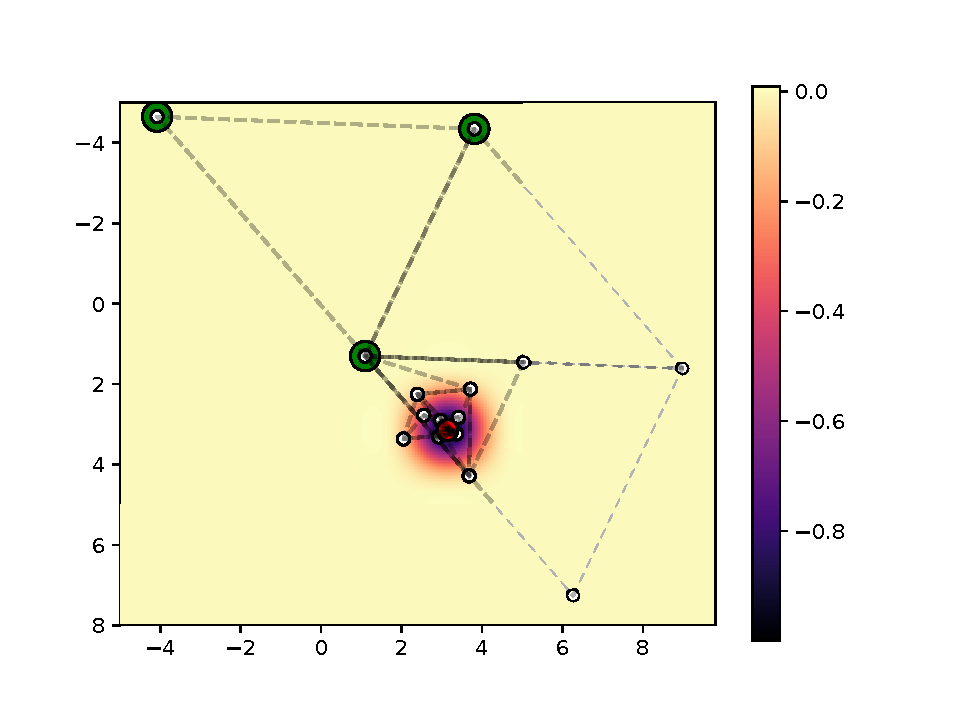
\includegraphics[width = .45\textwidth,trim={1cm 0 1cm 1.2cm}, clip]{Immagini/AbsoluteEasom1.pdf}} 
	\subfloat[]{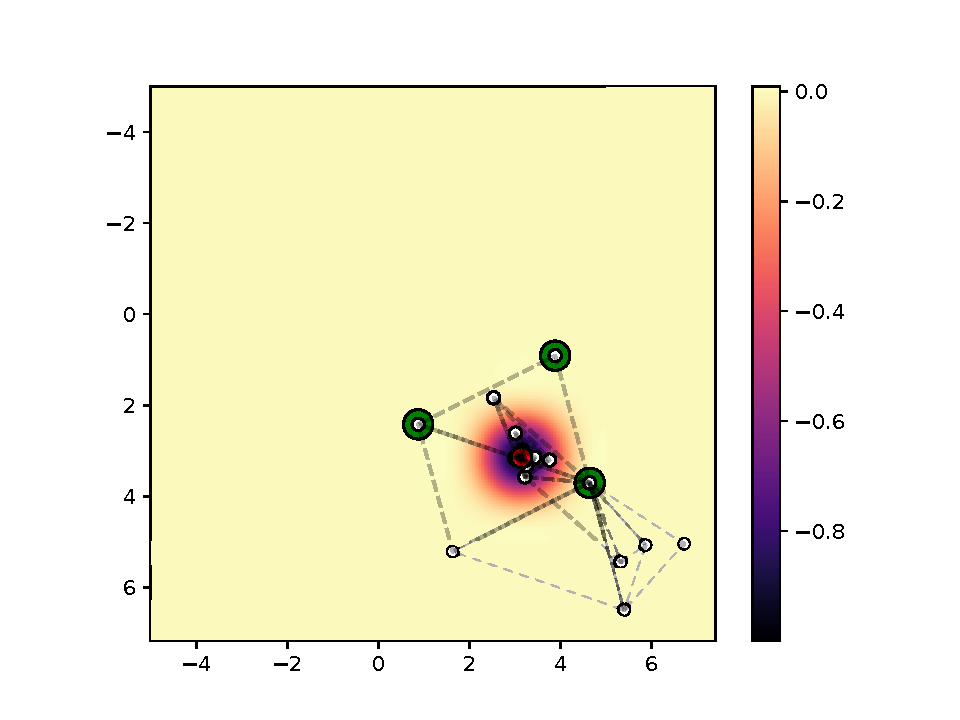
\includegraphics[width =  .45\textwidth,trim={1cm 0 1cm 1.2cm}, clip]{Immagini/AbsoluteEasom2.pdf}}\\
	\subfloat[]{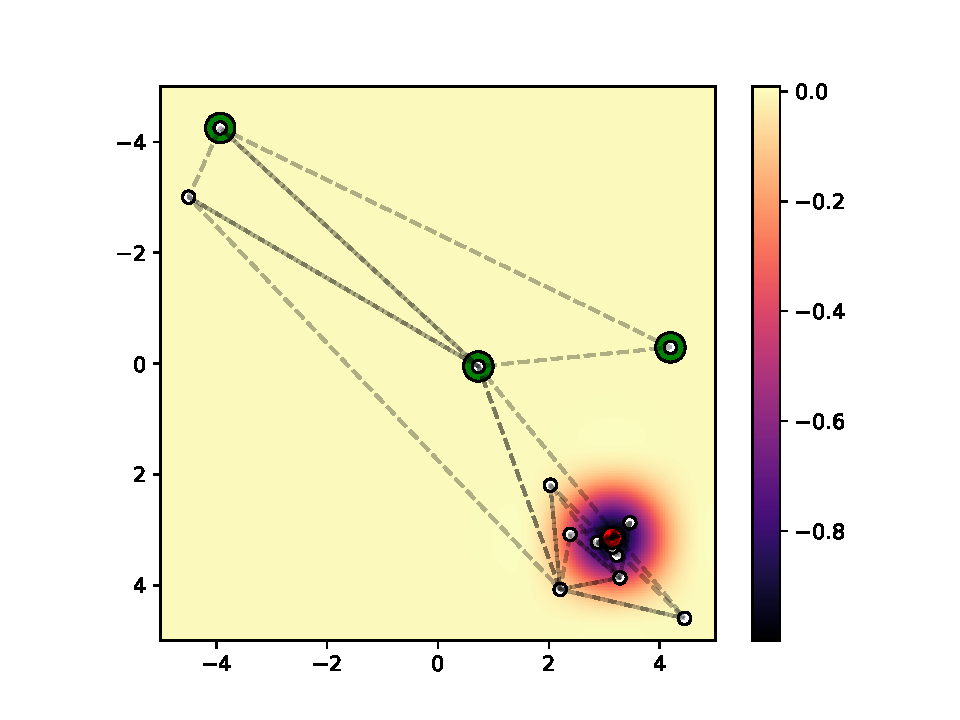
\includegraphics[width = .45\textwidth,trim={1cm 0 1cm 1cm}, clip]{Immagini/AbsoluteEasom3.pdf}}
	\subfloat[]{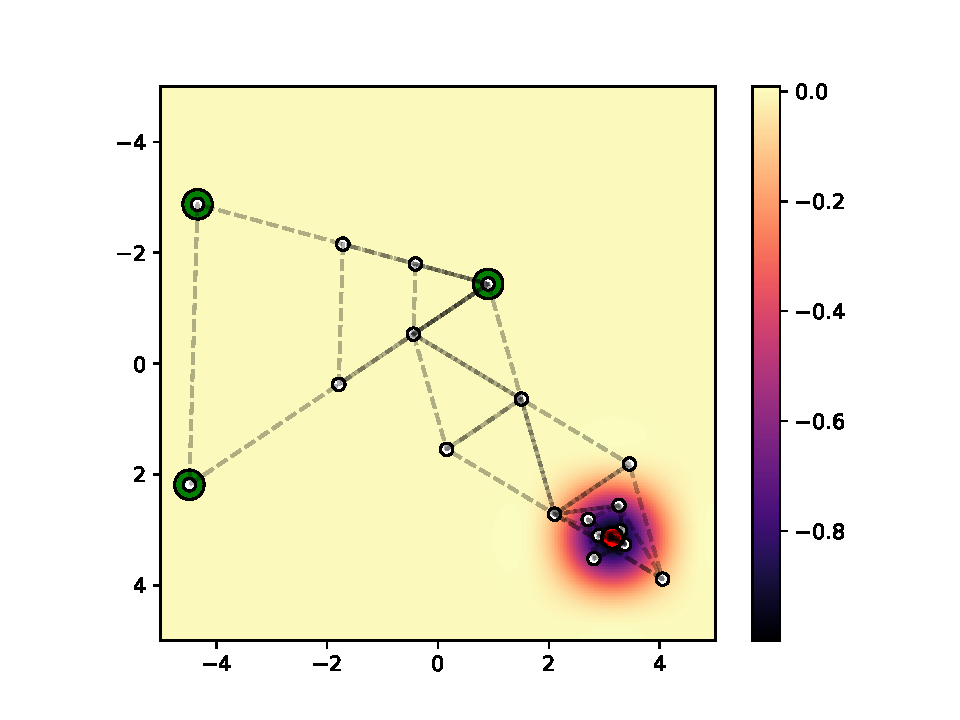
\includegraphics[width = .45\textwidth,trim={1cm 0 1cm 1cm}, clip]{Immagini/AbsoluteEasom4.pdf}} \\
	\subfloat[]{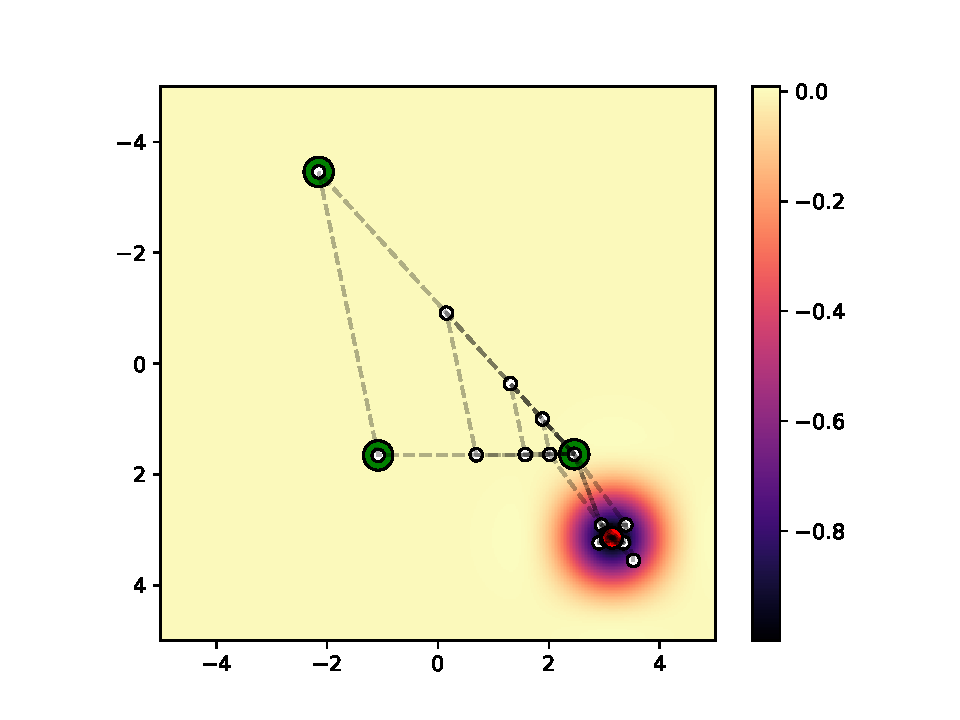
\includegraphics[width = .45\textwidth,trim={1cm 0 1cm 1cm}, clip]{Immagini/AbsoluteEasom5.pdf}}
	\subfloat[]{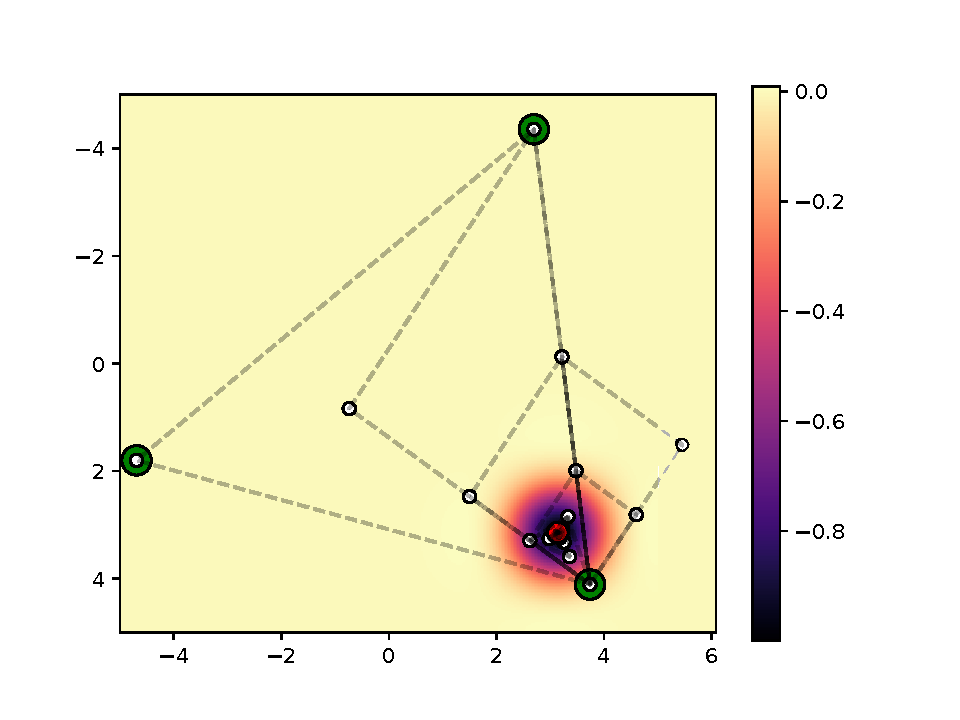
\includegraphics[width = .45\textwidth,trim={1cm 0 1cm 1cm}, clip]{Immagini/AbsoluteEasom6.pdf}}
	\label{fig:AbsoluteEasom}
\end{figure}

\begin{figure}
	\centering
	\caption{Sei istanze in cui il simplesso ha individuato dei minimi locali sul plateau della funzione di Easom.}
	
	\subfloat[]{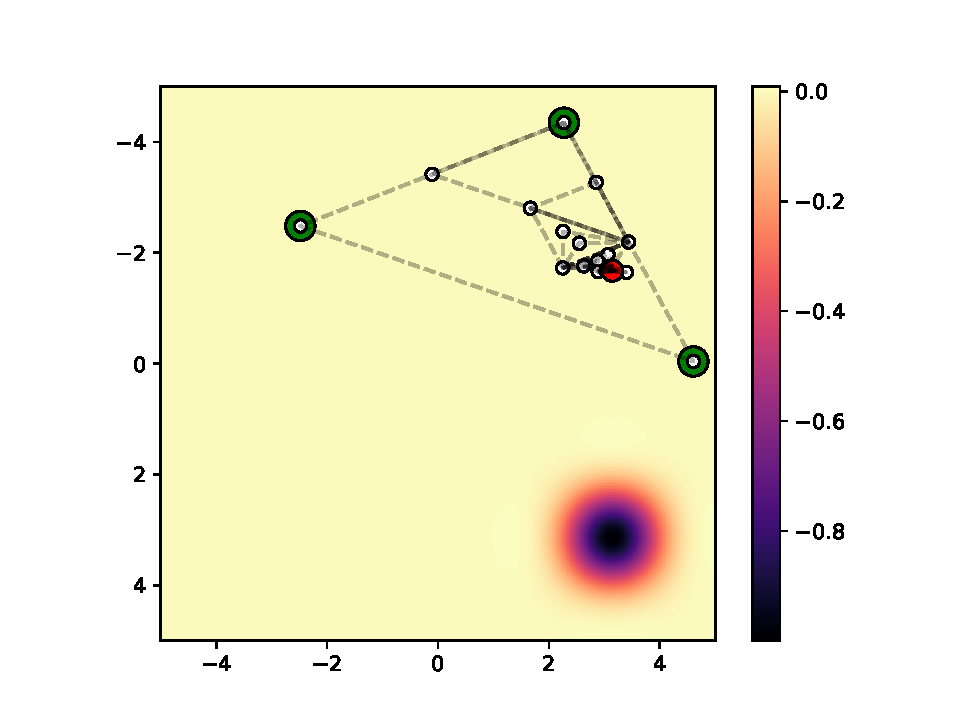
\includegraphics[width = .45\textwidth,trim={1cm 0 1cm 1cm}, clip]{Immagini/RelativeEasom1.pdf}} 
	\subfloat[]{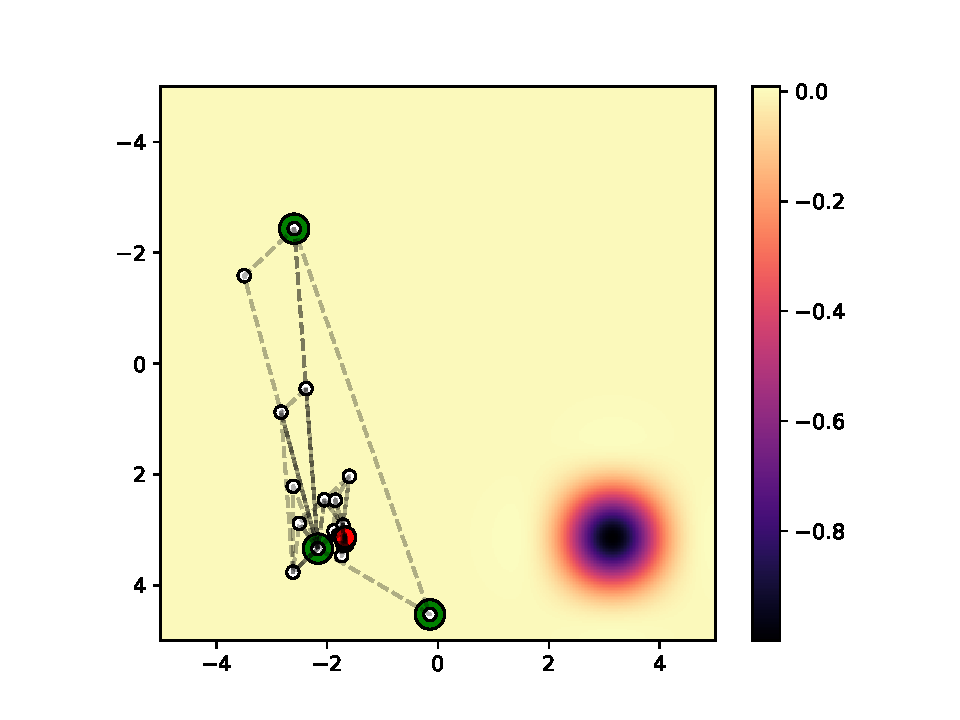
\includegraphics[width = .45\textwidth,trim={1cm 0 1cm 1cm}, clip]{Immagini/RelativeEasom2.pdf}}\\
	\subfloat[]{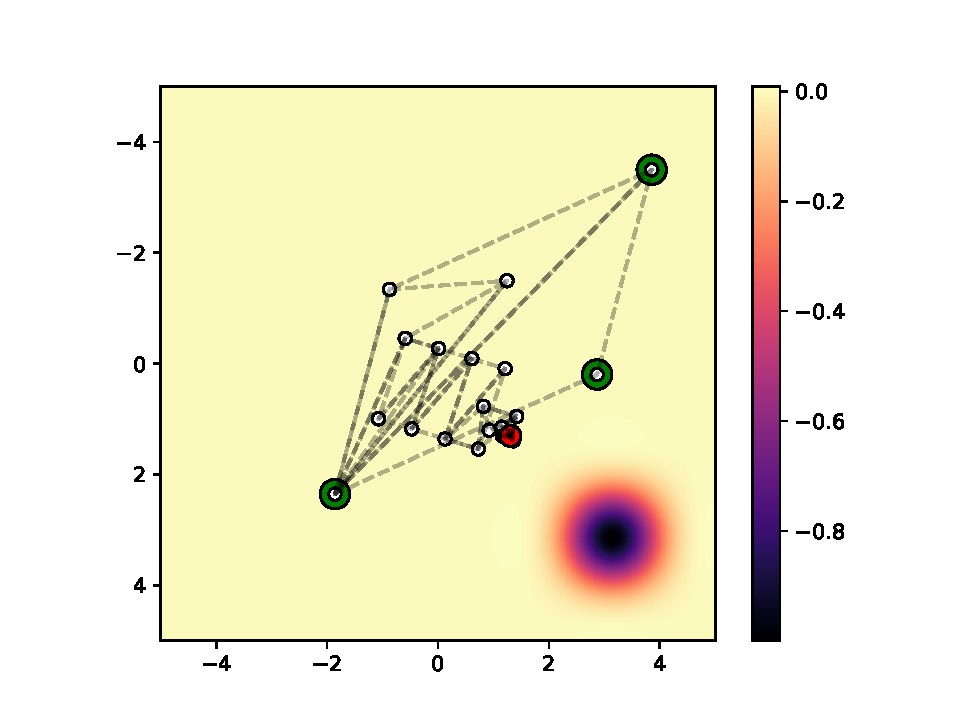
\includegraphics[width = .45\textwidth,trim={1cm 0 1cm 1cm}, clip]{Immagini/RelativeEasom3.pdf}}
	\subfloat[]{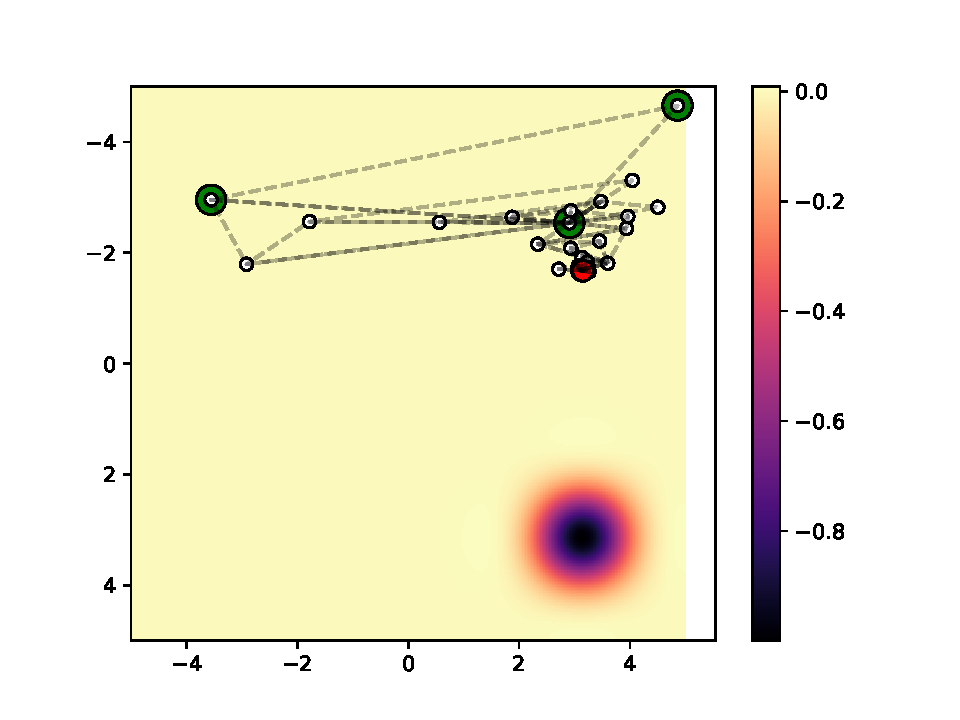
\includegraphics[width = .45\textwidth,trim={1cm 0 1cm 1cm}, clip]{Immagini/RelativeEasom4.pdf}} \\
	\subfloat[]{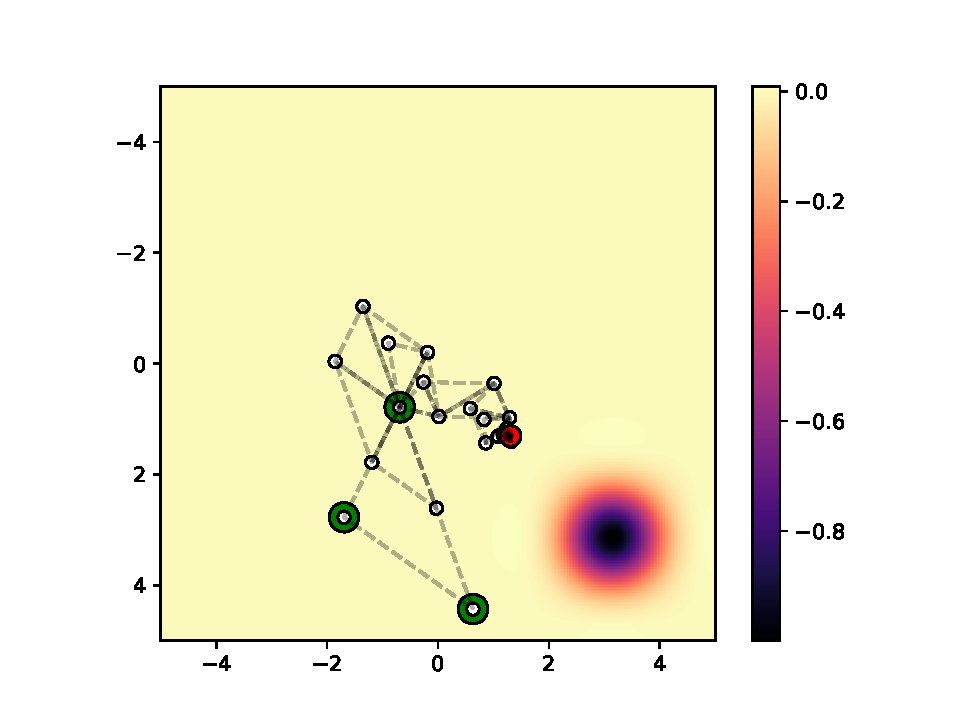
\includegraphics[width = .45\textwidth,trim={1cm 0 1cm 1cm}, clip]{Immagini/RelativeEasom5.pdf}}
	\subfloat[]{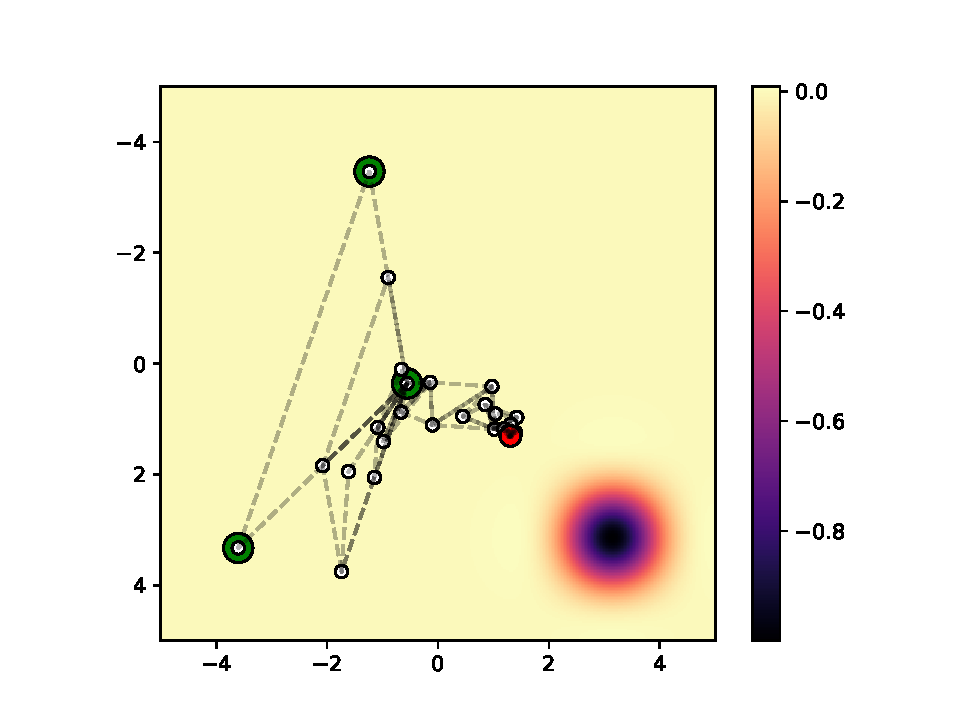
\includegraphics[width = .45\textwidth,trim={1cm 0 1cm 1cm}, clip]{Immagini/RelativeEasom6.pdf}}
	\label{fig:RelativeEasom}
\end{figure}

\newpage

\subsection*{Funzione di Goldstein-Price}

Anche in questo caso le coordinate iniziali dei vertici sono state generate casualmente nell'intervallo uniforme $\![-5,5]$. Il minimo locale globale è noto essere $f(3,4) = 1$, ragion per cui tale area di ricerca ci è sembrata senz'altro adeguata.\\

\noindent I grafici in \figurename~\ref{fig:Goldstein} evidenziano chiaramente una \emph{vallata circolare} puntualmente selezionata dall'evoluzione del simplesso. Su di essa effettivamente risiede il minimo globale: si tratta di una circonferenza centrata in $(0,0)$ e con raggio $R=5$. In particolare tutte le istanze della routine hanno trovato convergenza in due minimi: quello globale e uno locale nei dintorni di $(5,0)$.\\

\noindent Tali risultati appaiono del tutto ragionevoli se confrontati con il grafico in scala logaritmica riportato in \figurename~\ref{fig:GoldsteinLog}, che evidenzia appunto la struttura della corona circolare individuata dall'evoluzione del simplesso: si tratta di un vallata ad anello con fondo sostanzialmente piatto, tranne che per una "cresta" di minimi locali posizionati circa nel primo quadrante; i due più profondi sembrano essere proprio quelli selezionati dalla nostra routine.

\vfill

\begin{figure}[h!]
	\centering
	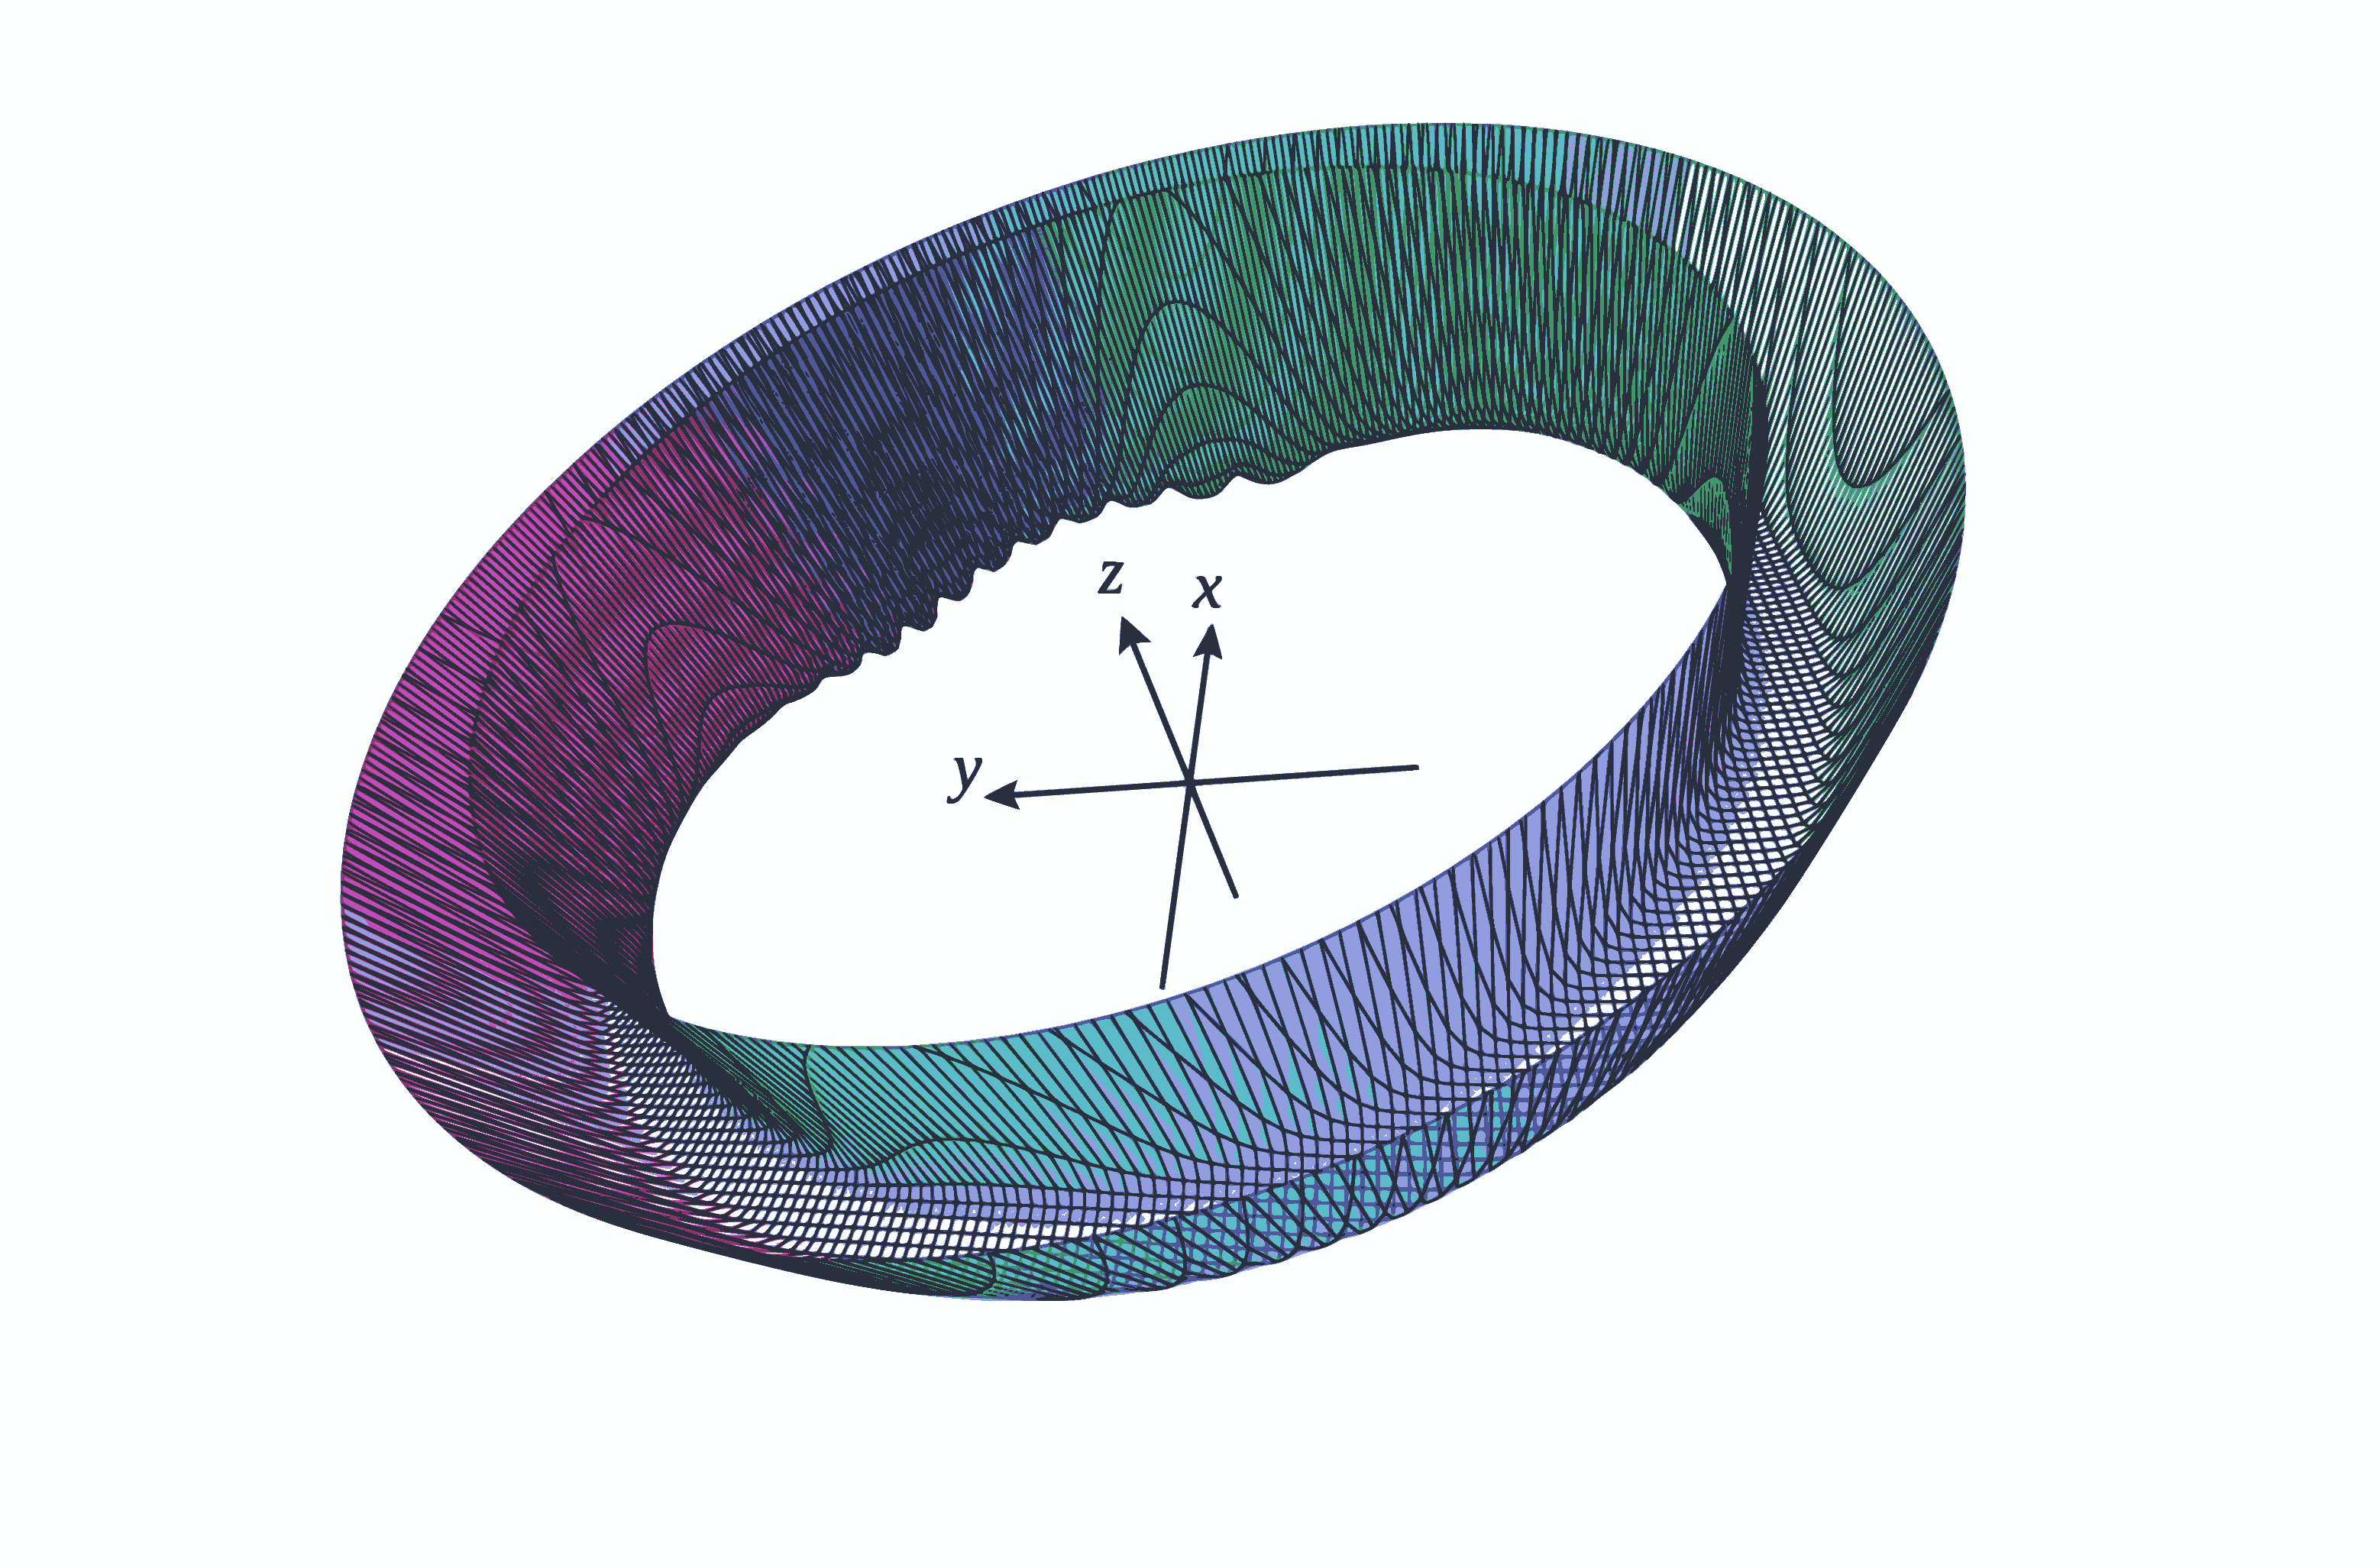
\includegraphics[width=1\linewidth, trim={5cm 5cm 5cm 1cm}, clip]{Immagini/GoldsteinLog.pdf}
	\caption{Grafico logaritmico della \emph{vallata circolare} in cui si trova il minimo globale della funzione di Goldstein-Price.}
	\label{fig:GoldsteinLog}
\end{figure}

\vfill

\begin{figure} 
	\centering
	\caption{Sei istanze che evidenziano la \emph{vallata circolare} della funzione di Goldstein-Price. In particolare (a), (c) e~(f) hanno selezionato il minimo globale $f(3,4) = 1$. La {colormap} è in scala logaritmica.}
	
	\subfloat[]{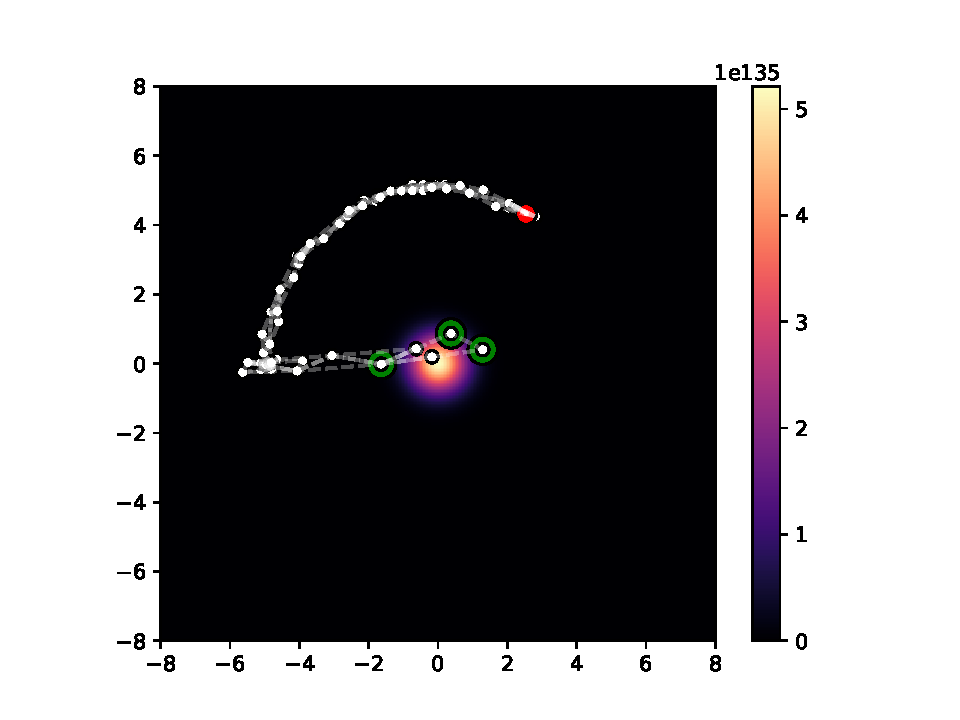
\includegraphics[width = .45\textwidth,trim={1cm 0 1cm 1cm}, clip]{Immagini/Goldstein1.pdf}} 
	\subfloat[]{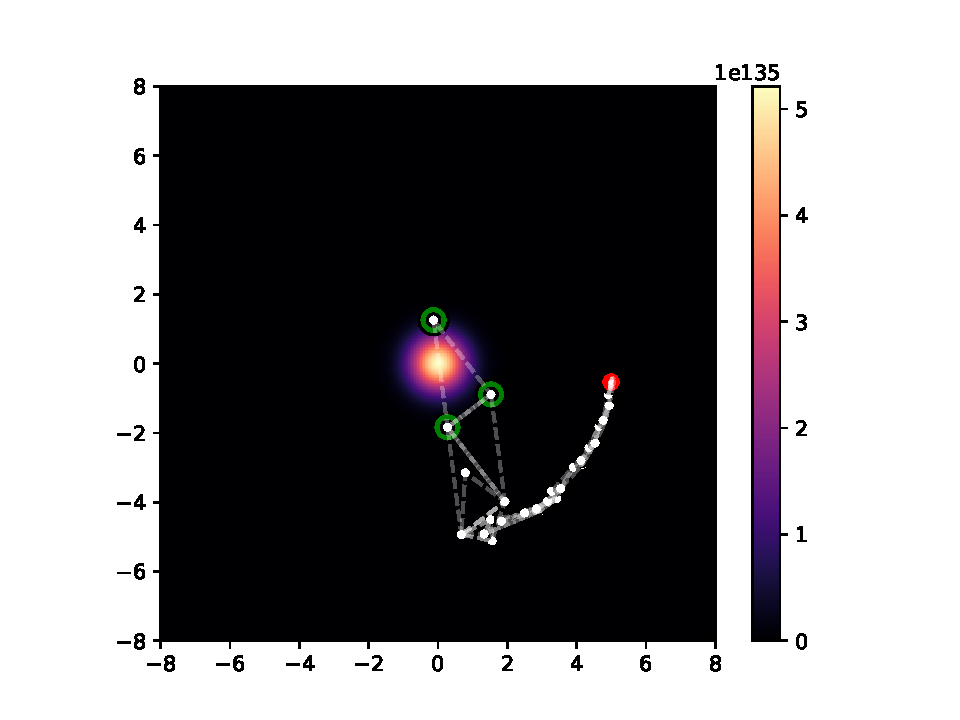
\includegraphics[width = .45\textwidth,trim={1cm 0 1cm 1cm}, clip]{Immagini/Goldstein2.pdf}}\\
	\subfloat[]{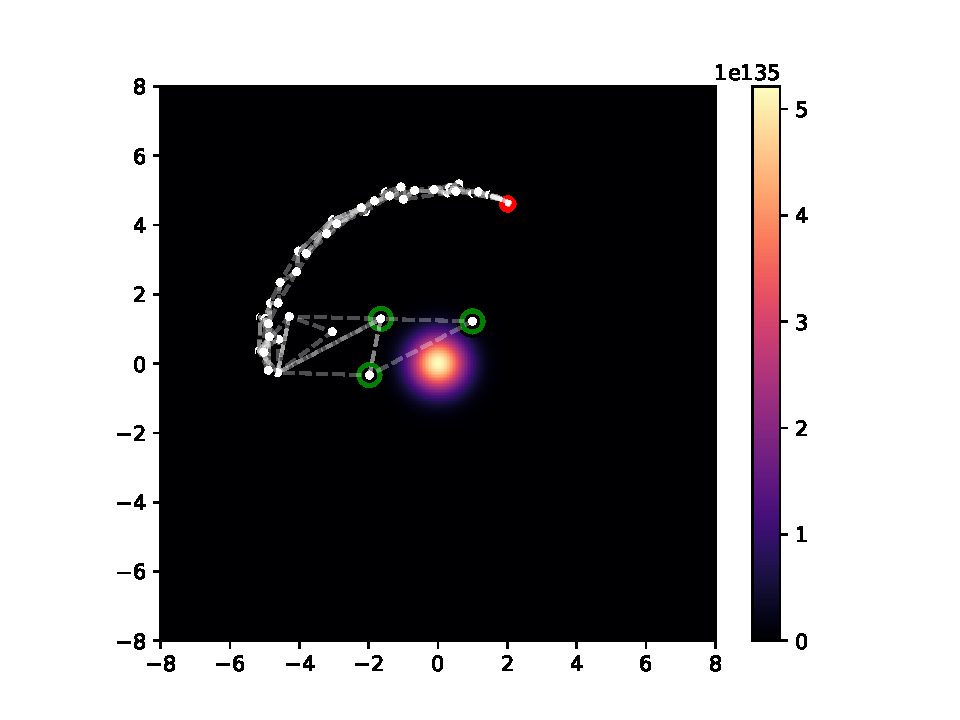
\includegraphics[width = .45\textwidth,trim={1cm 0 1cm 1cm}, clip]{Immagini/Goldstein3.pdf}}
	\subfloat[]{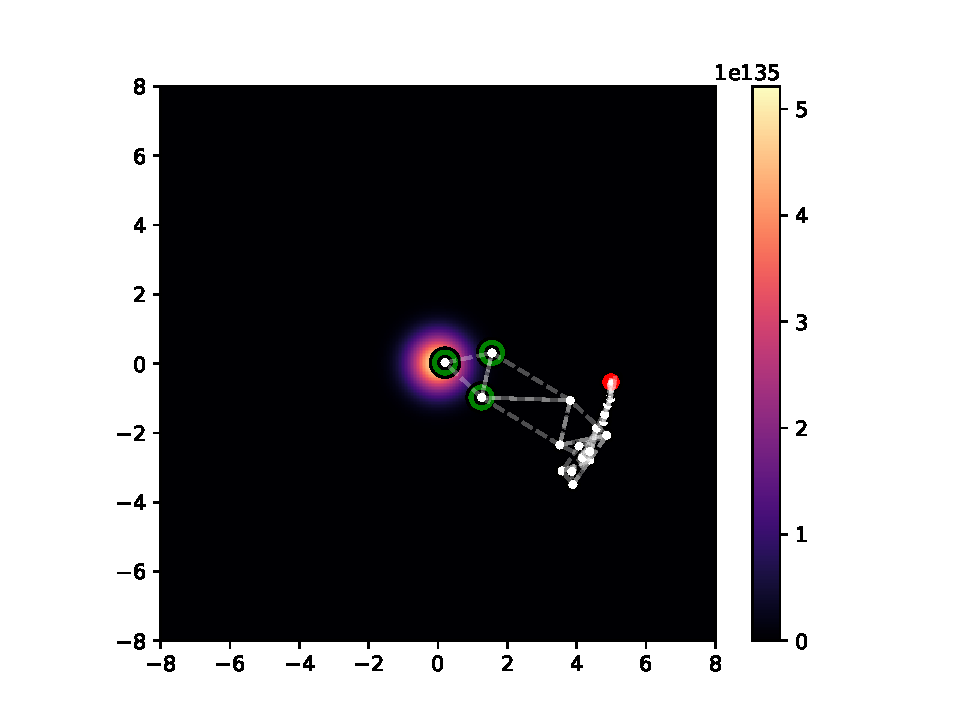
\includegraphics[width = .45\textwidth,trim={1cm 0 1cm 1cm}, clip]{Immagini/Goldstein4.pdf}} \\
	\subfloat[]{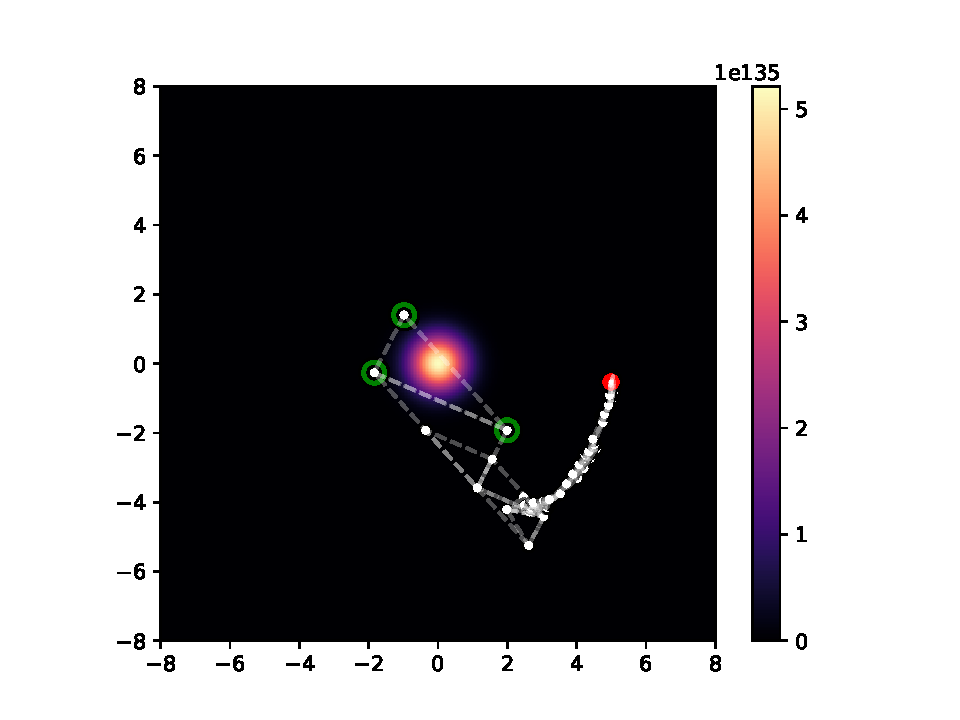
\includegraphics[width = .45\textwidth,trim={1cm 0 1cm 1cm}, clip]{Immagini/Goldstein5.pdf}}
	\subfloat[]{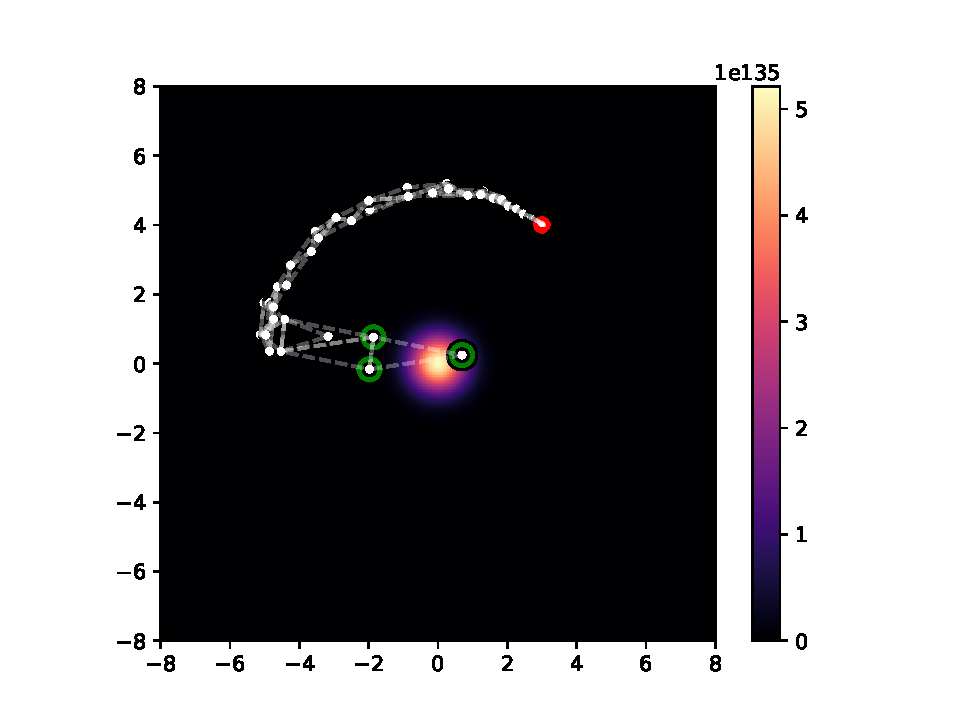
\includegraphics[width = .45\textwidth,trim={1cm 0 1cm 1cm}, clip]{Immagini/Goldstein6.pdf}}
	\label{fig:Goldstein}
\end{figure}

\newpage

\subsection*{Funzione di Bukin Nr.~6}

In \figurename~\ref{fig:EasomPlot} è riportato il grafico della funzione Nr.6 di Bukin. \`E evidente la presenza di una "cresta" di minimi locali posizionati lungo una fascia che interseca perpendicolarmente l'asse $\vec{x}$  nell'origine.\\

\noindent Estraendo coordinate uniformi  nella regione asimmetrica $x\in[-5,5]$, $y\in[-12,12]$ ne abbiamo individuati vari (Cfr. \figurename~\ref{fig:RelativeBukin}), anche relativamente lontani dal centro della fascia. Ne dedurremmo che i bordi della "cresta" non siano monotoni, anche se rimane il dubbio che in questo caso l'algoritmo implementato soffra di qualche criticità: il simplesso è sempre arrivato a convergere su intorni dati da una tolleranza di $\varepsilon=10^{-5}$ e valori inferiori hanno sempre prodotto tempi di calcolo eccessivamente prolungati.\\

\noindent Per quanto riguarda il minimo globale della funzione, posizionato lontano dalla cresta, in $\mathbf{x}_0 = (-10,1)$, abbiamo designato una regione stretta e mirata per la generazione dei vertici iniziali del simplesso - doppio intervallo uniforme $x\in[-12,-8]$, $y\in[0,3]$ - che ci ha permesso di arrivare ad approssimare con buona accuratezza il risultato:

\begin{align*}
\mathbf{x}_1 = (-9.94965119,  0.98995562) \enspace\enspace &\Longrightarrow \enspace\enspace f(\mathbf{x}_1) = 0.0005071942778401883\\
\mathbf{x}_2 = (-9.95151164,  0.99032607) \enspace\enspace &\Longrightarrow \enspace\enspace f(\mathbf{x}_2) = 0.0005075673516130408\\
\mathbf{x}_3 = (-9.95538255,  0.99109576) \enspace\enspace &\Longrightarrow \enspace\enspace f(\mathbf{x}_3) =0.0005122552638696298\\
\end{align*}

\noindent Il grafico dell'istanza che ha selezionato tali valori è riportato in \figurename~\ref{fig:AbsoluteBukin}.\\

\bigskip

\begin{figure}[h!]
	\centering
	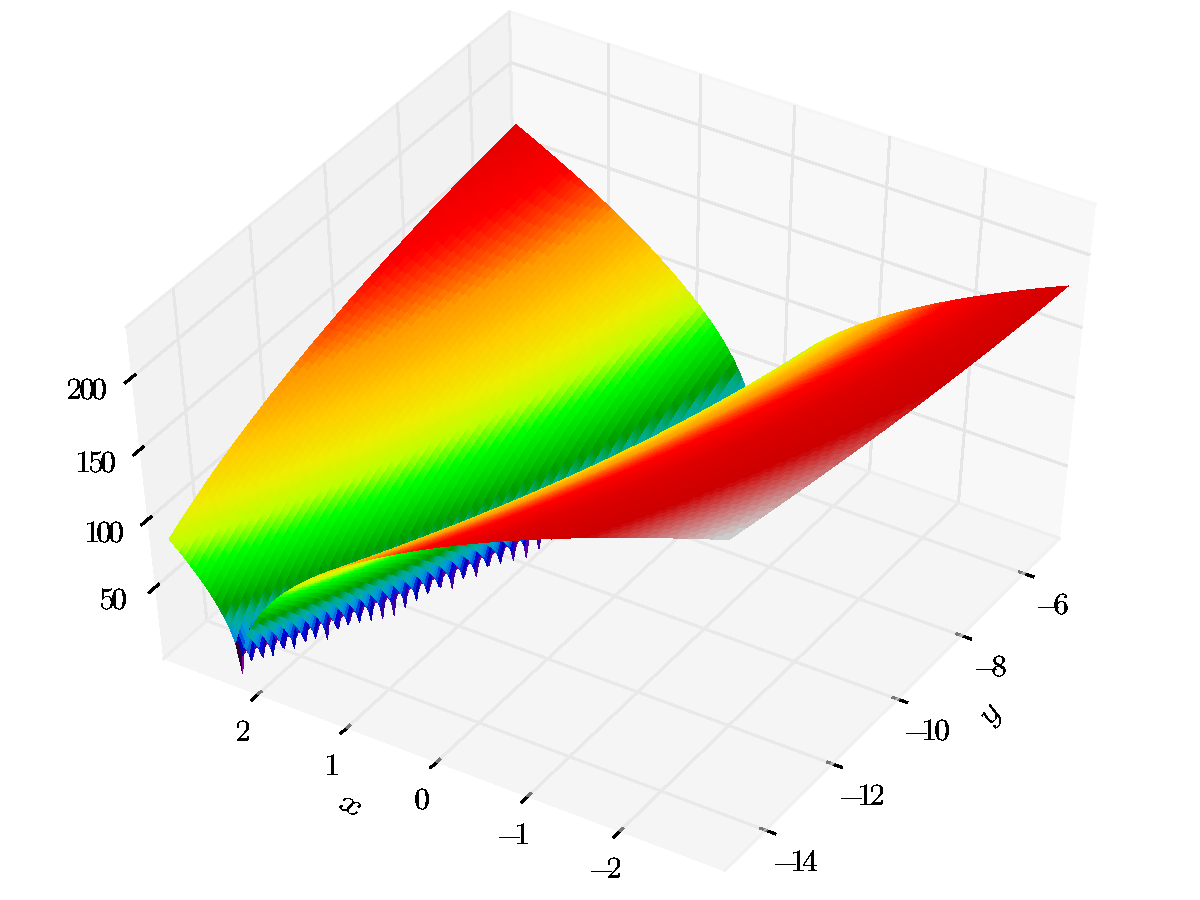
\includegraphics[width=0.85\linewidth]{Immagini/Bukin_function_6.pdf}
	\caption{Grafico 3D della funzione di Bukin Nr.~6. Da \texttt{Wikipedia} (Cfr. la nota a pié di pagina~\pageref{WikipediaFootnote}).}
	\label{fig:BukinPlot}
\end{figure}

\begin{figure}
	\centering
	\caption{Sei istanze mirate alla ricerca dei minimi locali sulla "cresta" della funzione Nr.6 di Bukin.}
	\subfloat[]{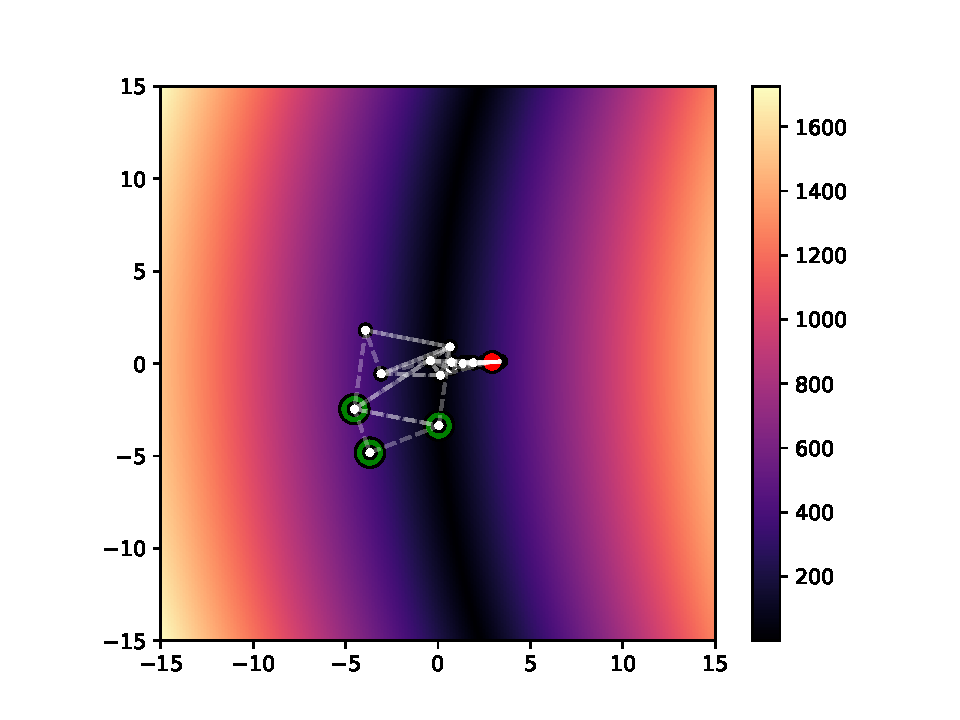
\includegraphics[width = .45\textwidth,trim={1cm 0 1cm 1cm}, clip]{Immagini/RelativeBukin1.pdf}} 
	\subfloat[]{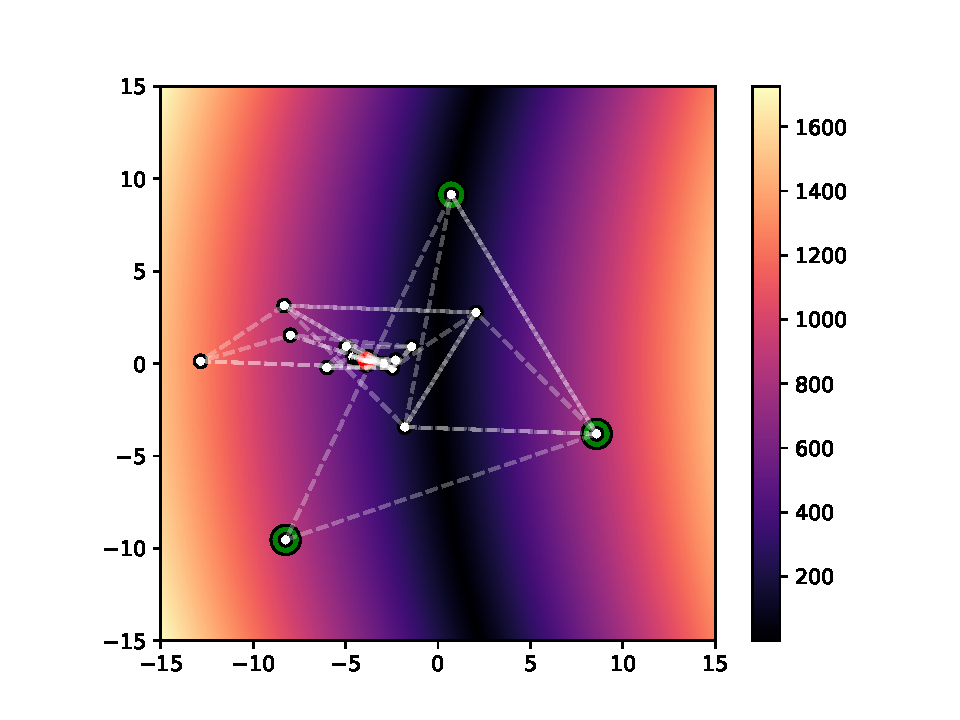
\includegraphics[width = .45\textwidth,trim={1cm 0 1cm 1cm}, clip]{Immagini/RelativeBukin2.pdf}}\\
	\subfloat[]{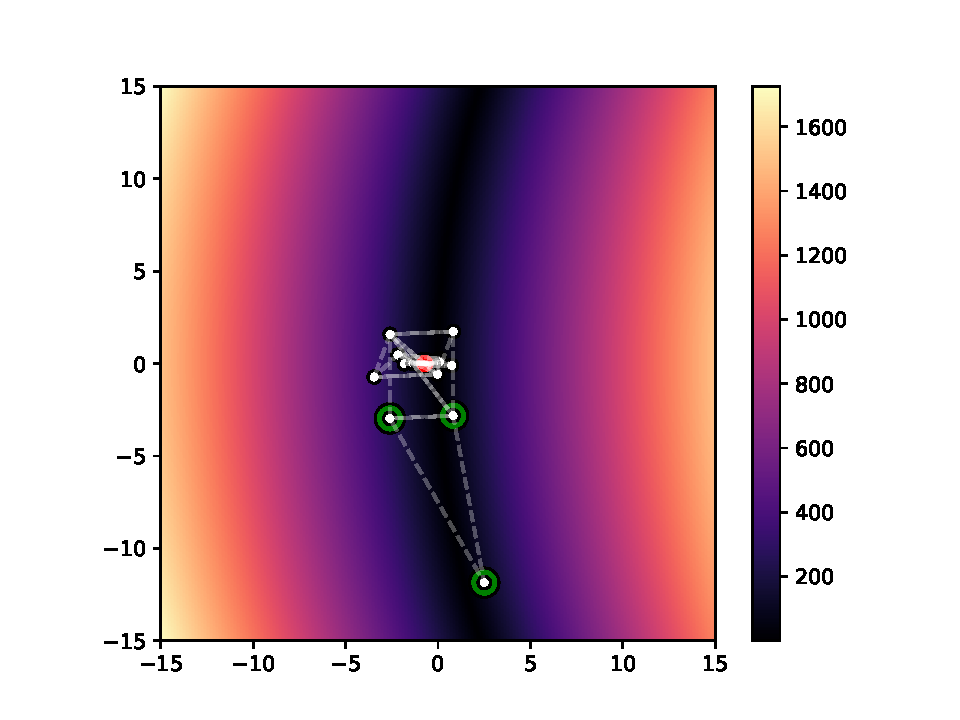
\includegraphics[width = .45\textwidth,trim={1cm 0 1cm 1cm}, clip]{Immagini/RelativeBukin3.pdf}}
	\subfloat[]{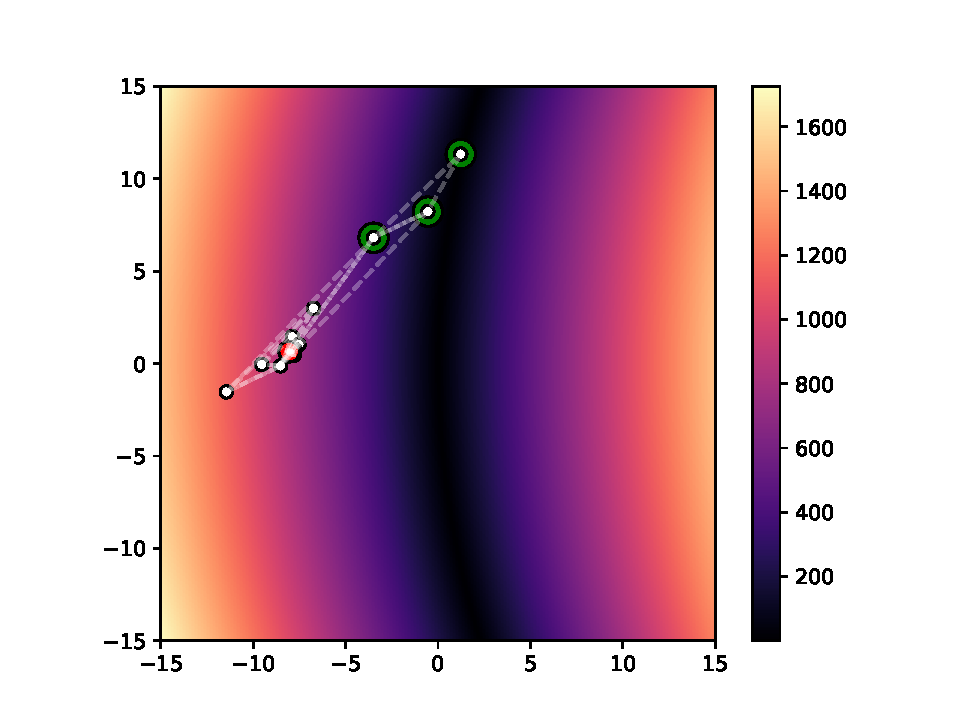
\includegraphics[width = .45\textwidth,trim={1cm 0 1cm 1cm}, clip]{Immagini/RelativeBukin4.pdf}} \\
	\subfloat[]{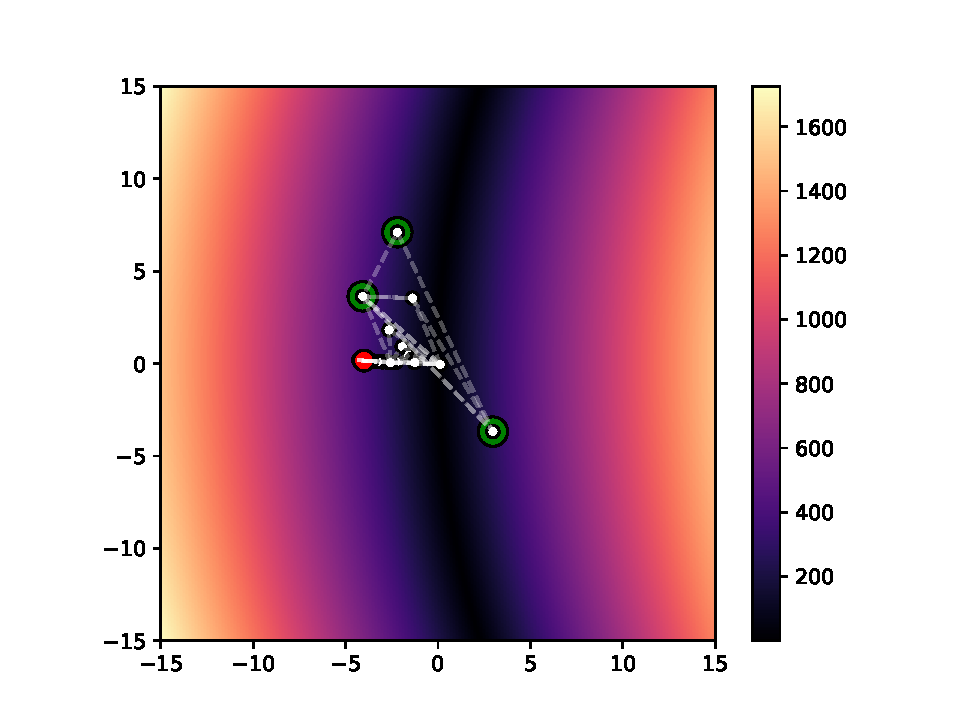
\includegraphics[width = .45\textwidth,trim={1cm 0 1cm 1cm}, clip]{Immagini/RelativeBukin5.pdf}}
	\subfloat[]{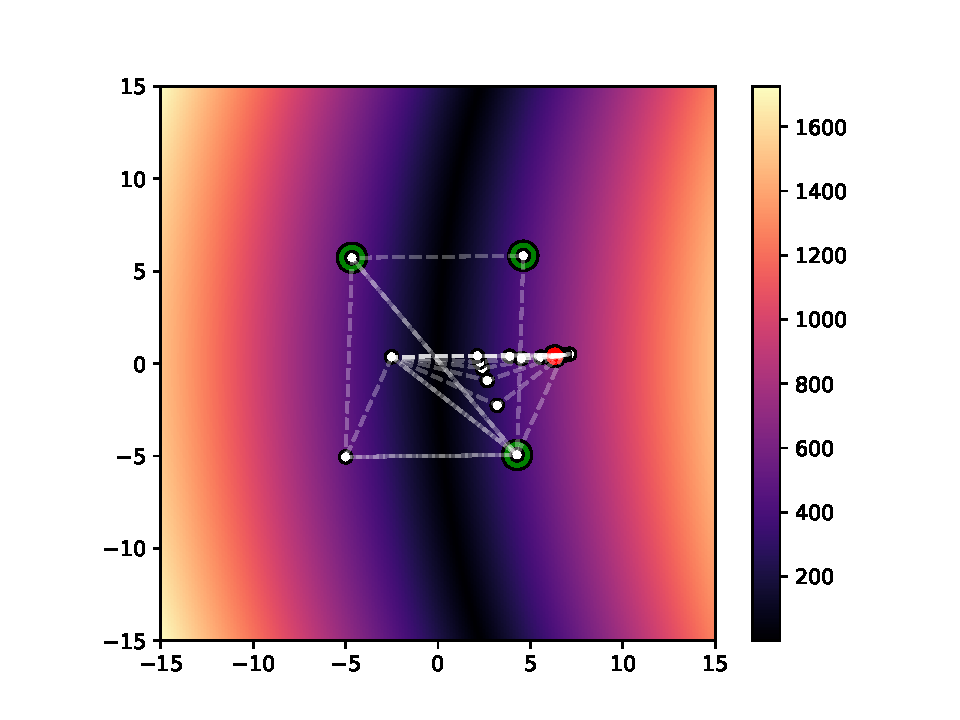
\includegraphics[width = .45\textwidth,trim={1cm 0 1cm 1cm}, clip]{Immagini/RelativeBukin6.pdf}}
	\label{fig:RelativeBukin}
\end{figure}

\begin{sidewaysfigure}
	\centering
	\caption{Ricerca del minimo globale della funzione Nr.~6 di Bukin.}
	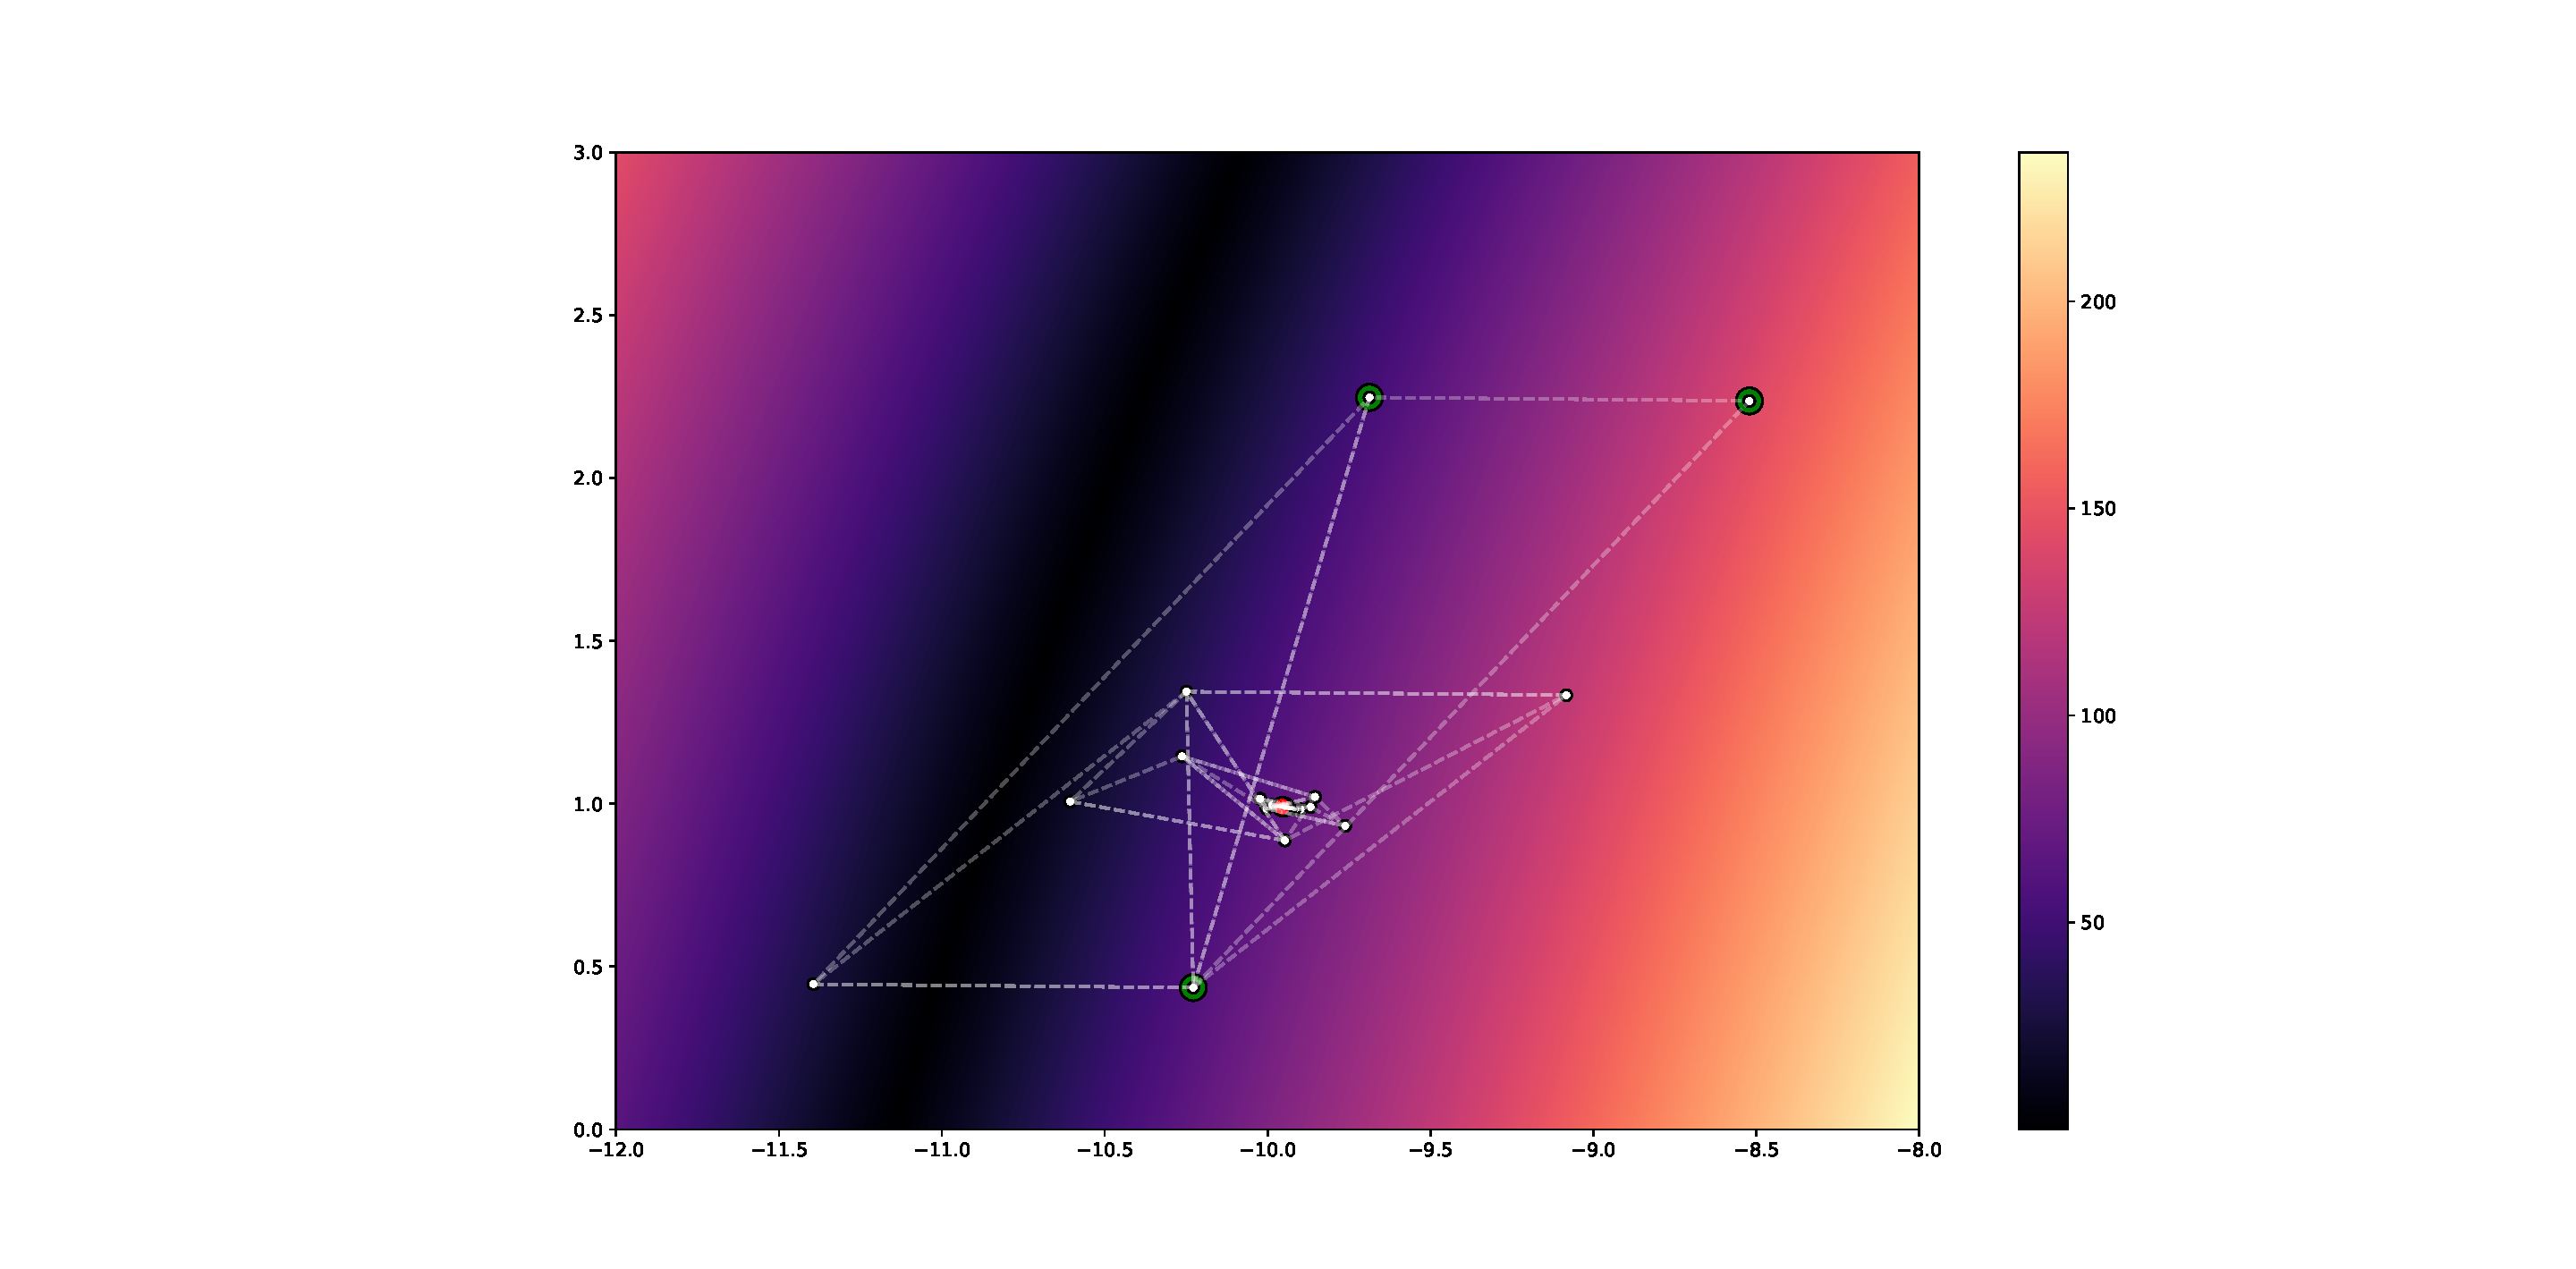
\includegraphics[width=\textwidth, trim={10cm 2cm 8cm 2cm}, clip]{Immagini/AbsoluteBukinBig.pdf}
	\label{fig:AbsoluteBukin}
\end{sidewaysfigure}

\newpage

\subsection*{Funzione di Booth}
\bigskip
La funzione di Booth è unimodale e convessa e in quanto tale presenta un unico minimo globale: $f(1,3) = 0$. Un~suo grafico è riportato in \figurename~\ref{fig:BoothPlot}.\\

\noindent In questa situazione l'algoritmo di Nelder-Mead è estremamente efficiente e si può generare il simplesso iniziale in una regione vasta a piacere. Noi abbiamo estratto le coordinate dei vertici nel doppio intervallo uniforme $[-15,15]$.\\

\noindent In \figurename~\ref{fig:Booth} sono riportati i grafici relativi a sei istanze della routine, ognuna delle quali ha dato convergenza al punto ottimo (entro $\varepsilon = 10^{-15}$ ) dopo qualche decina di passi.\\

\vfill

\begin{figure}[h!]
	\centering
	\includegraphics[width=\linewidth]{Immagini/Booth_function.pdf}
	\caption{Grafico 3D della funzione di Booth. Da \texttt{Wikipedia} (Cfr. la nota a pié di pagina~\pageref{WikipediaFootnote}).}
	\label{fig:BoothPlot}
\end{figure}

\vfill

\begin{figure}
	\centering
		\caption{Sei istanze in cui il simplesso è andato a convergere sul minimo globale della funzione di Booth.}
	\subfloat[]{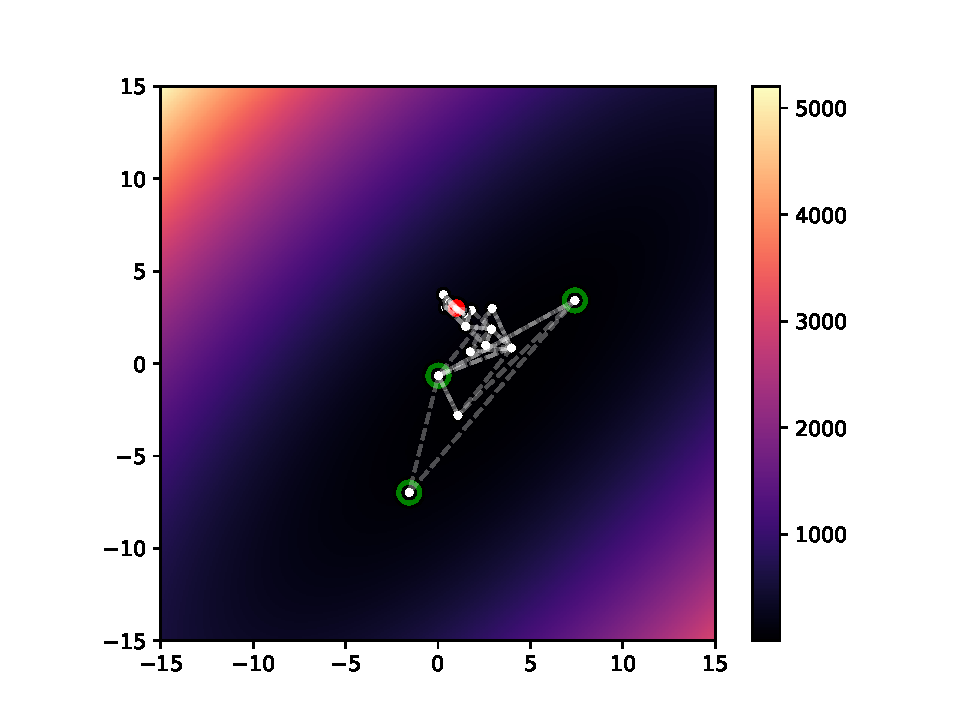
\includegraphics[width = .45\textwidth,trim={1cm 0 1cm 1cm}, clip]{Immagini/Booth1.pdf}} 
	\subfloat[]{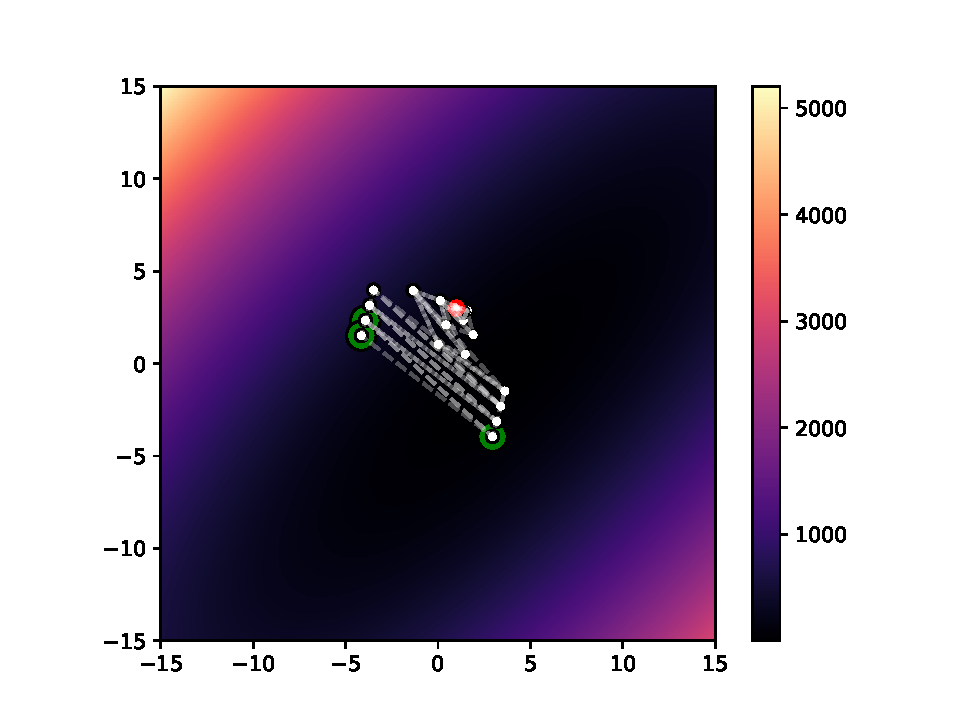
\includegraphics[width = .45\textwidth,trim={1cm 0 1cm 1cm}, clip]{Immagini/Booth2.pdf}}\\
	\subfloat[]{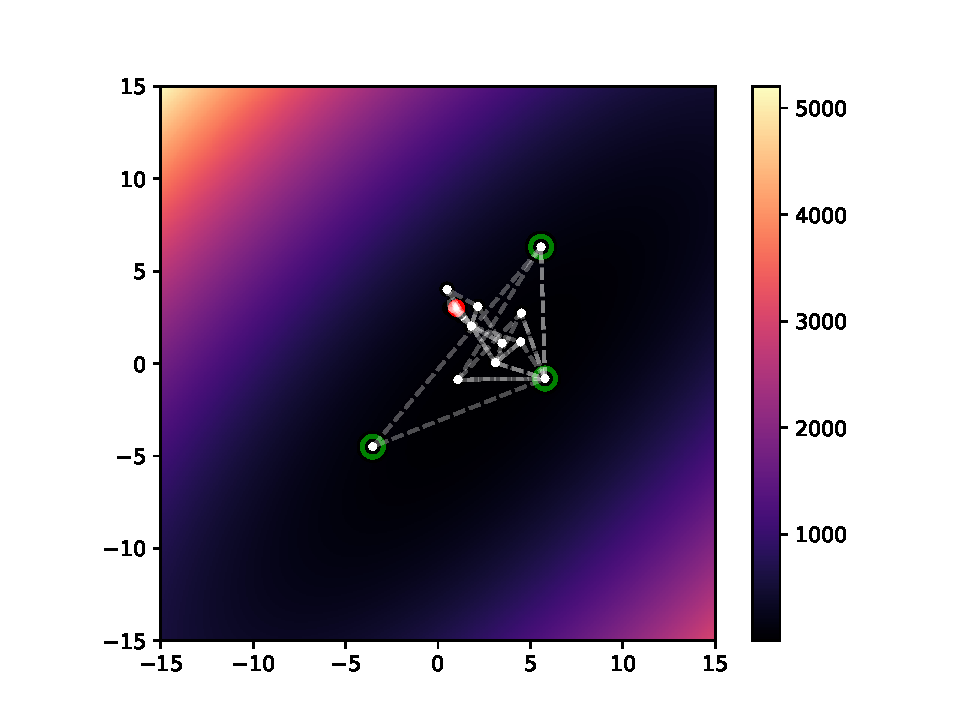
\includegraphics[width = .45\textwidth,trim={1cm 0 1cm 1cm}, clip]{Immagini/Booth3.pdf}}
	\subfloat[]{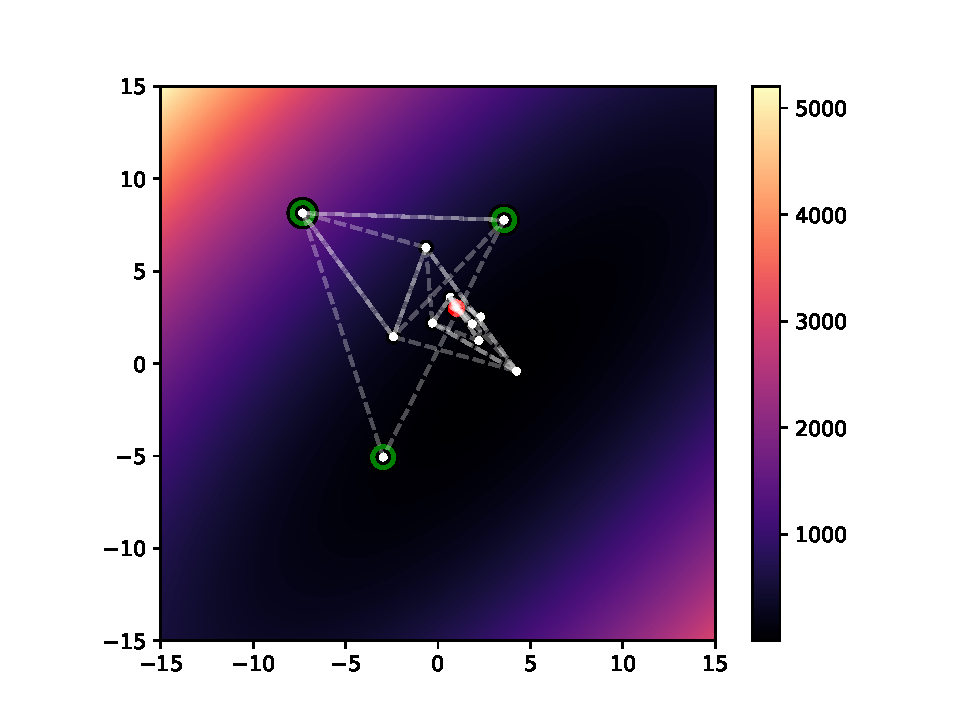
\includegraphics[width = .45\textwidth,trim={1cm 0 1cm 1cm}, clip]{Immagini/Booth4.pdf}} \\
	\subfloat[]{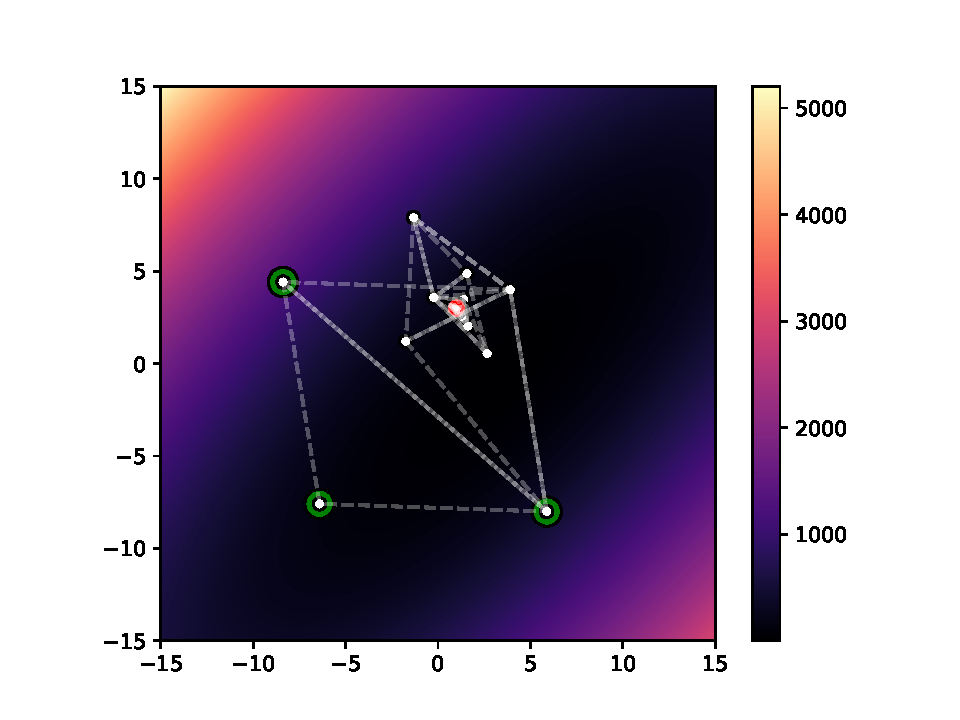
\includegraphics[width = .45\textwidth,trim={1cm 0 1cm 1cm}, clip]{Immagini/Booth5.pdf}}
	\subfloat[]{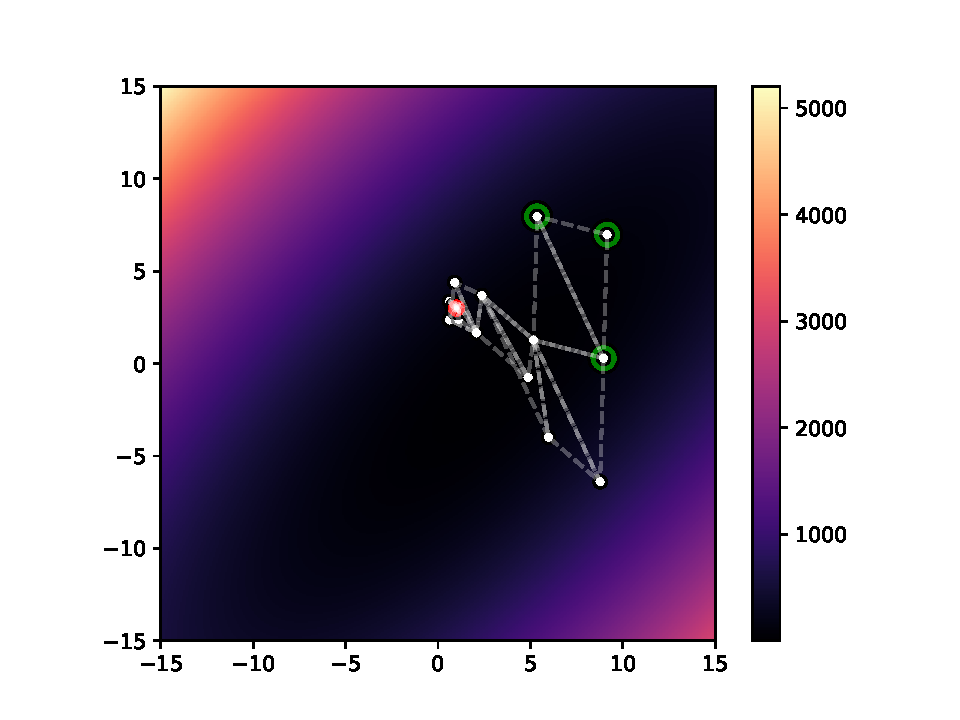
\includegraphics[width = .45\textwidth,trim={1cm 0 1cm 1cm}, clip]{Immagini/Booth6.pdf}}
	\label{fig:Booth}
\end{figure}

\newpage